% This template is intended to write a thesis using Latex at TI, RWTH.
% It supports bibtex and acronyms, which need a special toolchain building
% the document. Modern editors support such custom toolchains. Using acronyms
% needs the command makeglossaries to run, which requires a running Perl
% installation.

% The title of thesis can be set in three different fonts. Define the command
% of the font to use
% Standard sarif font. Works on all systems
% \def\titlefontStandardSerif{}
% Standard san sarif font. Works on all systems
\def\titlefontStandardSanSerif{}
% Special sarif font. Some viewers cannot display the font, if the document is
% created using latex (see below). Using pdflatex makes no problems. However
% this font makes the titlepage look interesting and is chosen as default.
%\def\titlefontSpecial{}

% One of these two toolchains are recommended. Use version a, if used graphics
% are *.eps/*.ps. Otherwise use version b. Both toolchains are intended to create
% a pdf and tested in the linux system accessible to students.
% '%' is the name of this file, i.e. 'thesis'.

% Version a
%  latex -synctex=1 -interaction=nonstopmode %.tex
%  bibtex %.aux
%  makeglossaries %
%  latex -synctex=1 -interaction=nonstopmode %.tex
%  dvips -o %.ps %.dvi
%  ps2pdf -dEmbedAllFonts=true %.ps

% Version b
%  pdflatex -synctex=1 -interaction=nonstopmode %.tex
%  bibtex %.aux
%  makeglossaries %
%  pdflatex -synctex=1 -interaction=nonstopmode %.tex

% In the following adapt the commands to your needs.
\author{Philipp Braun}
\title{Design of Adversarial Inputs for Deep Neural Networks using Iterative Approximations}
% For the titlepage the title needs to be split into 3 or 4 lines. If the fourth line is needed,
% use \titlelineA. Lines B and D are highlighted and should contain the important part of the title.
\def\titlelineA{Design of Adversarial Inputs for Deep Neural Networks using Iterative Approximations}
\def\titlelineB{Entwurf bösartiger Eingaben für tiefe neuronale Netze \\ mittels iterativer Approximationen}
% Further information
\def\thesistypegerman{Bachelorarbeit}
\def\thesistype{Bachelor Thesis}
\def\supervisor{M.Sc. Emilio R. Balda} % Not professor

% The header includes all packages and defines many macros. All packages are tested to run
% under the latex-distribution (texlive) available in the student's linux system. The
% macros are neither complete nor the only way to typeset math. However they have shown to
% be useful while writing a thesis. Both packages and macros can be deleted or commented
% if not needed.

%!TEX root = thesis.tex
% The basic document settings
\documentclass[11pt,a4paper,twoside,abstract=on]{scrreprt}
% If you have problems compiling this template, try adding the following
% package in order to allow for more packages to be included
% A possible error could look like this:
% "No room for a new \dimen \newdimen \MPscratchDim"
%\usepackage{etex}

% Compatibility issues solved
% \usepackage{scrhack}

\usepackage{amsmath}
\usepackage[makeroom]{cancel}
\usepackage[ngerman,english]{babel}
\usepackage{setspace}
\usepackage{subcaption}

\usepackage{sansmath}

\DeclareMathOperator*{\argmax}{argmax}

% Further (Koma) options:
% Table of references and indices in TOC
\KOMAoptions{bibliography = totoc}
\KOMAoptions{index = totoc}
% Behaviour of paragraphs (full = empty line, false = ident)
\KOMAoptions{parskip = full}
% Draw line under page header
\KOMAoptions{headsepline = true}
% New chapters always start on right page
\KOMAoptions{open = right}

% Page formatting
\setlength{\evensidemargin}{0.5cm}
\setlength{\oddsidemargin}{0.5cm}
\setlength{\topmargin}{0.5cm}
\setlength{\textwidth}{15cm}

% Pre formatted pagestyle
\pagestyle{headings}

% Font and language
%\usepackage{german}
%\usepackage[latin1]{inputenc}


%\usepackage[ngerman]{babel}
%\usepackage{lmodern} % Better font
%\usepackage[utf8]{inputenc}
%\usepackage[T1]{fontenc}

\usepackage{ifxetex}

\ifxetex
  \usepackage{fontspec}
  \usepackage{polyglossia}
  \setmainlanguage[spelling=new, latesthyphen=true]{german}
\else
  \usepackage[T1]{fontenc}
  \usepackage[utf8]{inputenc}
  \usepackage[ngerman]{babel}
  \usepackage{lmodern}
\fi

%\definecolor{darkgray}
%\font{Adobe Caslon Pro}
% Easier quotation marks

%\usepackage [autostyle, english = british]{csquotes}
%\MakeOuterQuote{"}

% Mandatory for some bib styles
%\usepackage{natbib}

% Maths:
\usepackage{amsfonts, amsmath, amsthm, amscd, amssymb, array, bm, mathtools}
\usepackage{nicefrac}
\usepackage{cases} % For sub numbered cases
\numberwithin{equation}{section} % Equation umbering chapter.section.equation
\usepackage{bigints} % Big integral signs

% Bring color into Latex
\usepackage[svgnames]{xcolor}
\usepackage{colortbl}
\definecolor{hellgrau}{rgb}{0.9,0.9,0.9}

% Several graphics packages
% General graphics
\usepackage{graphicx}
\usepackage{grffile}
\usepackage{lipsum}
%\usepackage{flafter}
% LaPrint (exports matlab figures for latex)
\usepackage{color, psfrag}
% ps-graphics
\usepackage{pstricks,pst-plot,pst-node}
% TIKZ
\usepackage{tikz}
\usetikzlibrary{arrows,matrix,positioning}
% Set the path for figure files
\graphicspath{{./figures/}}
\def\layersep{2.5cm}
\tikzset{basic/.style={draw,fill=blue!50,text width=1em,text badly centered}}
\tikzset{input/.style={basic,circle}}
\tikzset{weights/.style={basic,rectangle,minimum width=0.7cm, minimum height=0.6cm}}
\tikzset{functions/.style={basic,circle,fill=blue!50}}


% Prevent figures from floating too much
\usepackage[section]{placeins}

% SI-Units
\usepackage{siunitx}

% Algorithms
% \usepackage{algpseudocode,algorithmicx}
% \renewcommand{\algorithmicrequire}{\textbf{Input:}}
%\renewcommand{\algorithmicensure}{\textbf{Output:}}

\usepackage{algorithm,algpseudocode}
% \usepackage[ruled]{algorithm2e}

% Better tabulars, enables thicker lines
\setlength{\doublerulesep}{0pt}
\usepackage{multirow} % Multirows in tabulars
\usepackage{longtable, tabu} % Flexible tabulars i.e. page breaks and horizontal fill
\newtabulinestyle{mydashline=on 1.5pt off 2pt}
\tabulinesep=1mm

% Creating an index
%\usepackage{makeidx}
% Adding items to index more comfortably
%\newcommand{\idx}[1]{#1\index{#1}}

% Abbrevations
% Note that the abbrevations support commands like \ac{acronym} and the creation
% of a list of acronyms. In order to create this list, the document needs to be
% compiled as follows (includes optional bibtex). Use pdflatex or latex as preferred
%     (pdf)latex thesis.tex
%     bibtex thesis.aux
%     makeglossaries thesis
%     (pdf)latex thesis.tex
%\usepackage[nomain, toc, shortcuts]{glossaries}
% Removes a dot at the end of every description
%\renewcommand*{\glspostdescription}{}
%\loadglsentries{acronym.tex}
%\bibliographystyle{alphadin}



% Links in PDFs
\usepackage{hyperref}
\hypersetup{colorlinks=false, pdfborder={0 0 0}}
\makeatletter
\hypersetup{pdftitle = \@title}
\hypersetup{pdfauthor = \@author}
\makeatother
\hypersetup{pdfsubject = \thesistypegerman}

% Automatic referencing (e.g. \ref{...} creates figure 2.1.3)
\usepackage[english]{cleveref}
\renewcommand{\figurename}{Figure}%
% No eq. in front of equations
\crefformat{equation}{#2(#1)#3}
\Crefformat{equation}{#2(#1)#3}

% Some math macros:
% Operators
\newcommand{\modulo}{\ensuremath{\mbox{mod }}}
\newcommand{\abs}[1]{\ensuremath{\left\vert #1 \right\vert}}
\newcommand{\card}[1]{\ensuremath{\left\vert #1 \right\vert}}
\newcommand{\norm}[2]{\ensuremath{\left\Vert #1 \right\Vert_{#2}}}
\newcommand{\divisor}{\ensuremath{\mathrm{div}}}
\newcommand{\ord}{\ensuremath{\mathrm{ord}}}
\newcommand{\supp}{\ensuremath{\mathrm{supp}}}
\newcommand{\ggt}{\ensuremath{\mathrm{ggt}}}
\newcommand{\charac}{\ensuremath{\mathrm{char}}}
\newcommand{\ud}{\ensuremath{\,\mathrm{d}}} % Integral d (dx, dy, etc.)
\newcommand{\ppart}[1]{\ensuremath{\left[#1\right]^{+}}}
\newcommand{\npart}[1]{\ensuremath{\left[#1\right]^{-}}}
\DeclareMathOperator{\diag}{diag}
\newcommand{\vecop}{\ensuremath{\operatorname{\mathbf{vec}}}}

% Sets
\newcommand{\Z}{\ensuremath{\mathbb{Z}}}
\newcommand{\N}{\ensuremath{\mathbb{N}}}
\newcommand{\J}{\ensuremath{\mathbb{J}}}
\newcommand{\HD}{\ensuremath{\mathbb{P}}}
\newcommand{\D}{\ensuremath{\mathbb{D}}}
\newcommand{\R}{\ensuremath{\mathbb{R}}}  % Real numbers
\newcommand{\Rp}{\ensuremath{\R_{\geq 0}}} % Nonnegative real numbers
\newcommand{\CO}{\ensuremath{\mathcal{O}}}
\newcommand{\F}{\ensuremath{\mathbb{F}}}
\newcommand{\I}{\ensuremath{\mathcal{I}}}
\newcommand{\allsubsets}[1]{\mathfrak{B}(#1)}
\newcommand{\X}{\ensuremath{\mathbb{X}}}
\newcommand{\Y}{\ensuremath{\mathbb{Y}}}

% Optimization
\newcommand{\minimize}{\ensuremath{&\operatorname{minimize} &&}}
\newcommand{\minimizex}[1]{\ensuremath{&\underset{#1}{\operatorname{minimize}}&&}}
\newcommand{\maximize}{\ensuremath{&\operatorname{maximize} &&}}
\newcommand{\maximizex}[1]{\ensuremath{&\underset{#1}{\operatorname{maximize}}&&}}
\newcommand{\st}{\ensuremath{&\operatorname{subject~to}&&}}
\newcommand{\stff}{\ensuremath{&&&}}

% For vectors and matrices
\renewcommand{\vec}[1]{\ensuremath{\bm{\MakeLowercase{#1}}}}
\newcommand{\mat}[1]{\ensuremath{\bm{\MakeUppercase{#1}}}}
\newcommand{\vecidx}[2]{\ensuremath{\MakeLowercase{#1}_{#2}}}
\newcommand{\vecidxB}[2]{\ensuremath{\left[#1\right]_{#2}}}
\newcommand{\vecidxBppart}[2]{\ensuremath{\left[#1\right]^{+}_{#2}}}
\newcommand{\vecidxBnpart}[2]{\ensuremath{\left[#1\right]^{-}_{#2}}}
\newcommand{\matidx}[3]{\ensuremath{\MakeLowercase{#1}_{#2 #3}}}
\newcommand{\matidxB}[3]{\ensuremath{\left[#1\right]_{#2 #3}}}
\newcommand{\matidxBppart}[3]{\ensuremath{\left[#1\right]_{#2 #3}^{+}}}
\newcommand{\transp}[1]{\ensuremath{#1^{\top}}}
\newcommand{\inv}[1]{\ensuremath{#1^{-1}}}
\newcommand{\pinv}[1]{\ensuremath{#1^{\dagger}}}
\newcommand{\opt}[1]{\ensuremath{#1^{\star}}}
\newcommand{\unitvec}{\vec{e}}
\newcommand{\identmat}{\mat{i}}
\newcommand{\zerovec}[1]{\vec{0}_{#1}}
\newcommand{\zeromat}[2]{\mat{0}_{#1\times #2}}
\newcommand{\onevec}[1]{\vec{1}_{#1}}
\newcommand{\onemat}[2]{\mat{1}_{#1\times #2}}

% Logics
\newcommand{\logicnot}{\lnot}
\newcommand{\logicand}{\wedge}
\newcommand{\logicor}{\vee}
\newcommand{\logicxor}{\oplus}

% Colors
\newcommand{\bl}{\color{blue}}
\newcommand{\bk}{\color{black}}
\newcommand{\rd}{\color{red}}
\newcommand{\gr}{\color{green}}

\newcommand{\mcl}{\mathcal}

% Convert number 1 to 12 into corresponding months
%\newcommand{\monthword}[1]{\ifcase#1\or January\or February\or March\or April\or
%                                        May\or June\or July\or August\or
%                                        September\or October\or November\or December\fi}

%\makeglossaries   % -> run makeglossaries thesis
\makeindex


% Beginning of the real document
\begin{document}
\let\origref\ref % The original \ref command is now accessible by \origref
\let\ref\cref    % The command \ref uses \cref from the cleveref package now

% First pages with roman numbering
\pagenumbering{roman}

%!TEX root = thesis.tex
%******************************************************************************
% Some definitions
%******************************************************************************

% Command for generating a specific amount of whitespace
\newlength{\drop}
\drop=0.05\textheight % Define the command as 10% of the total text height

% Format of emphasized title line
\definecolor{rwthblue}{RGB}{37,83,161}

\def\emphtitleline{\huge\color{rwthblue}}
\def\nonemphtitleline{\large}

% Two lines at top and bottom of page
\def\twolinestop{ %
% \rule{\textwidth}{1pt}\par % Thick horizontal line
\vspace{2pt}\vspace{-\baselineskip} % Whitespace between lines
\rule{\textwidth}{0.4pt}\par % Thin horizontal line
}
\def\twolinesbottom{ %
\rule{\textwidth}{0.4pt}\par % Thick horizontal line
\vspace{2pt}\vspace{-\baselineskip} % Whitespace between lines
% \rule{\textwidth}{1pt}\par % Thin horizontal line
}

% The font of the title
% Standard serif
\ifdefined\titlefontStandardSerif
\def\titlefont{\normalfont}
\fi
% Standard san serif
\ifdefined\titlefontStandardSanSerif
\def\titlefont{\sffamily} %%% used font
\fi
% Special serif font. Name: Pacioli
\ifdefined\titlefontSpecial
\def\titlefont{\usefont{\encodingdefault}{cpc}{m}{n}\selectfont}
\fi

%******************************************************************************
% The real title page
%******************************************************************************

\begin{titlepage}
\vspace*{-30mm}
\begin{flushright}

\includegraphics{figures/rwth_ti_de_rgb.jpg}
\end{flushright}
\centering
%\twolinestop
\vspace{1.5\drop} % Whitespace between the top lines and title


\begin{center}
{ \titlefont\renewcommand{\baselinestretch}{1.70}\normalsize
{\emphtitleline \textbf{\titlelineA} } \\[0.7\baselineskip]
{\nonemphtitleline \titlelineB} \\
}

\vspace{1.2\drop} % Whitespace between the title and short horizontal line
%\rule{0.5\textwidth}{0.4pt}\par % Short horizontal line under the title
%\vspace{0.1\drop} % Whitespace between the thin horizontal line and the author name

\makeatletter
{\Large \titlefont{\@author}}\par % Author name
\makeatother

\end{center}

\vfill % Whitespace between the author name and publisher text
\vspace*{20mm}

%
\includegraphics{figures/Ti_black}\\[0.5\baselineskip] % Include a department/university logo
{\large \titlefont{Lehrstuhl für Theoretische Informationstechnik}}\\[0.5\baselineskip] % Institute
{\large \titlefont{RWTH Aachen University}}\par % Uni
%
%\vspace*{0.2\drop} % Whitespace
%
% \twolinesbottom
\end{titlepage}
%
\cleardoublepage

%******************************************************************************
% A second title page containing more information
%******************************************************************************

\thispagestyle{empty}
\begingroup
\vspace*{-30mm}
\begin{flushright}

\includegraphics{figures/rwth_ti_de_rgb.jpg}
\end{flushright}
\centering
% \twolinestop
\vspace{1.5\drop} % Whitespace between the top lines and title

\begin{center}
{ \titlefont\renewcommand{\baselinestretch}{1.70}\normalsize
{\emphtitleline \textbf{\titlelineA} } \\[0.7\baselineskip]
{\nonemphtitleline \titlelineB} \\
}

\vspace{1.2\drop} % Whitespace between the title and short horizontal line
%\rule{0.5\textwidth}{0.4pt}\par % Short horizontal line under the title
%\vspace{0.1\drop} % Whitespace between the thin horizontal line and the author name

\makeatletter
{\Large \titlefont{\@author}}\par % Author name
\makeatother

\end{center}

\vspace{2\drop}

\begin{center}
\textsf{Bachelorarbeit eingereicht an der Fakultät für} \\
\textsf{Elektrotechnik und Informationstechnik,}\\
\textsf{RWTH Aachen Universität}\\[0.5\baselineskip]
\textsf{geprüft von Univ.-Prof. Dr. rer. nat. Rudolf Mathar}\\[0.5\baselineskip]
%am \textsf{\today}\\[0.5\baselineskip] %\textsf{\monthword{\month}~\the\year}
\end{center}

\vfill % Whitespace between the author name and publisher text
\vspace*{20mm}
%
\includegraphics{figures/Ti_black}\\[0.5\baselineskip] % Include a department/university logo
{\large \titlefont{Lehrstuhl für Theoretische Informationstechnik}}\\[0.5\baselineskip] % Institute
{\large \titlefont{RWTH Aachen University}}\par % Uni

%
%\vspace*{0.2\drop} % Whitespace
%
% \twolinesbottom
\endgroup
%
\cleardoublepage

%!TEX root = thesis.tex
%******************************************************************************
% Assurance everything is single handed
%******************************************************************************
\begin{otherlanguage}{ngerman}

\begingroup
\thispagestyle{empty}
\begin{center}
	\large
	\textbf{Eidesstattliche Versicherung}
\end{center}

\vspace{0.5cm}

\begin{tabular}{@{}p{8cm}p{5.8cm}}
	\underline{\hspace{6cm}} & \underline{\hspace{5.8cm}} \\
	\vspace{0.02cm}Name, Vorname & \vspace{0.02cm}Matrikelnummer \\
\end{tabular}
\vspace{0.5cm}

Ich versichere hiermit an Eides Statt, dass ich die vorliegende {\thesistypegerman} mit dem Titel

{\makeatletter{\emph{{\@title}}}\makeatother}

selbständig und ohne unzulässige fremde Hilfe erbracht habe. Ich habe keine anderen als die angegebenen Quellen und Hilfsmittel benutzt. Für den Fall, dass die Arbeit zusätzlich auf einem Datenträger eingereicht wird, erkläre ich, dass die schriftliche und die elektronische Form vollständig übereinstimmen. Die Arbeit hat in gleicher oder ähnlicher Form noch keiner Prüfungsbehörde vorgelegen.

\vspace{0.3cm}

\begin{tabular}{@{}p{8cm}p{5.8cm}}
	\underline{\smash{Aachen, den \today}} & \underline{\hspace{5.8cm}}\\
	\vspace{0.02cm}Ort, Datum & \vspace{0.02cm}Unterschrift \\
\end{tabular}

\vspace{1cm}

\begin{small}
	\textbf{Belehrung:}

	\textbf{§ 156 StGB: Falsche Versicherung an Eides Statt}\\
	Wer vor einer zur Abnahme einer Versicherung an Eides Statt zuständigen Behörde eine solche Versicherung falsch abgibt oder unter Berufung auf eine solche Versicherung falsch aussagt, wird mit Freiheitsstrafe bis zu drei Jahren oder mit Geldstrafe bestraft.

	\textbf{§ 161 StGB: Fahrlässiger Falscheid; fahrlässige falsche Versicherung an Eides Statt}\\
	(1) Wenn eine der in den §§ 154 bis 156 bezeichneten Handlungen aus Fahrlässigkeit begangen worden ist, so tritt Freiheitsstrafe bis zu einem Jahr oder Geldstrafe ein.\\
	(2) Straflosigkeit tritt ein, wenn der Täter die falsche Angabe rechtzeitig berichtigt. Die Vorschriften des § 158 Abs. 2 und 3 gelten entsprechend
\end{small}

\vspace{0.3cm}

Die vorstehende Belehrung habe ich zur Kenntnis genommen:

\vspace{0.3cm}



\begin{tabular}{@{}p{8cm}p{5.8cm}}
	\underline{\smash{Aachen, den \today}} & \underline{\hspace{5.8cm}}\\
	\vspace{0.02cm}Ort, Datum & \vspace{0.02cm}Unterschrift \\
\end{tabular}

\endgroup
\cleardoublepage

\end{otherlanguage}

%******************************************************************************
% Abstract
%******************************************************************************

\begingroup
\def\abstractname{Abstract}
\begin{abstract}
\thispagestyle{plain}

In recent years, deep learning methods have gained popularity in various research areas.
Especially, data-driven businesses have rapidly adopted and deployed machine learning techniques that use neural networks.
Despite this fact, neural networks are internally often poorly understood. Therefore, the attack surface
as well as the accuracy of these systems is difficult to measure and assess. However, in autonomous driving, spam filters,
biometric authentication, algorithmic trading or medical applications precision of prediction systems is vital \cite{NeuralMed,ControlPipeline}.
Therefore, this thesis focuses on the creation of adversarial inputs for these networks. To find the
optimal input perturbation, different convex optimization techniques are introduced. Comparisons to previous research papers are drawn and
existing techniques improved through iterative approximations. Later on, experimentation results are presented to verify these
convex optimization techniques. Adversarial examples introduced in the simulations are often
indistinguishable from the original input images.
\end{abstract}
\endgroup

%******************************************************************************
% Acknowledgements
%******************************************************************************


\begingroup
\def\abstractname{Acknowledgements}
\begin{abstract}
\thispagestyle{plain}

I would first like to thank my thesis advisor M.Sc. Emilio R. Balda for teaching me the necessary skills for academic research and software development.
Getting used to tensorflow and various optimization techniques was quite a steep slope.
Furthermore, I would like to thank my friends and family for the endless support they have given me over the years of my studies.

\end{abstract}
\endgroup


\tableofcontents
\cleardoublepage


\chapter*{Acronyms}
\addcontentsline{toc}{chapter}{Acronyms}
\markboth{Accronyms}{Acronyms}

{\renewcommand{\arraystretch}{1.5}
\begin{longtabu}{l X}
\textsf{\textbf{DNN}} & Deep Neural Network \\
\textsf{\textbf{ReLu}} & Rectifier Linear Unit \\
\textsf{\textbf{GP}} & Gaussian Process \\
\textsf{\textbf{FCNN}} & Fully-Connected Neural Network \\
\textsf{\textbf{CNN}} & Convolutional Neural Network \\
\textsf{\textbf{AE}} & Autoencoder \\
\textsf{\textbf{VAE}} & Variation Autoencoder \\
\textsf{\textbf{NN}} & Neural Network \\
\textsf{\textbf{FGSM}} & Fast Gradient Sign Method \\
\textsf{\textbf{PSNR}} & Peak Signal-To-Noise Ratio \\
\textsf{\textbf{GAN}} & Generative Adversarial Network \\
\textsf{\textbf{MSE}} & Mean Squared Error \\
\end{longtabu}
}

\chapter*{Notation}
\addcontentsline{toc}{chapter}{Notation}
\markboth{Notation}{Notation}

{\renewcommand{\arraystretch}{1.5}
\begin{longtabu}{l X}
$\bm{x}$ & input for DNN layers \\
$\bm{y}$ & expected output based on the dataset \\
$\bm{b}$ & bias term \\
$f$ & output of the DNN \\
$L$ & maximum number of layers \\
$l$ & layer index \\
$\bm{W}$ & weight matrix \\
$\mcl{L}$ & loss or cost function \\
$\phi$ & activation function \\
$W$ & input dimension of the CNN \\
$F$ & filter size \\
$P$ & input padding \\
$S$ & stride or step size \\
$\bm{\eta}$ & input perturbation \\
$\epsilon$ & perturbation constraint \\
$N$ & number of iterations, pixels or last layer's dimension \\
$\bm{e}_k$ & canonical vector \\
$\bm{v}_{max}$ & eigenvector with maximum eigenvalue \\
$\mcl{S}$ & subset for a single pixel \\
$Z$ & input image depth \\
$S$ & number of subsets \\
$i_s^z$ & subset indices \\
$\bm{P}$ & used pixels during iterative solutions \\
\end{longtabu}
}


% The main part
\pagenumbering{arabic}
%!TEX root = thesis.tex
\chapter{Introduction}\label{sec:chapter}

\section{Neural Networks}

\begingroup
Neural networks are a set of algorithms, modeled loosely after human brains and are designed to recognize patterns \cite{DeepIntro}.
To recognize a specific pattern these networks need to be trained on large datasets to optimize the high number of model parameters.
This has led to a lot of research by data-driven companies like Google. Thus resulting in various breakthroughs in text processing engines, image recognition
and speech processing using Deep Neural Networks (DNNs) \cite{GoogleTranslation, AlexNet, SpeechRecognition}.

Unfortunately, these networks are also not fault-free. While prooving the fault tolerance of
mathematical techniques and algorithms is relatively simple, finding the hidden edge cases for DNNs is not.
Therefore, rigorous adversarial testing is necessary to avoid failures.
\endgroup


\section{Adversarial Examples}\label{sec:section}

\begingroup
Adversarial examples are inputs intentionally designed to change the output of a DNN. Often the perturbed
input images are almost indistinguishable from the original images.
Therefore, an attacker with
access to the input of a DNN is able to severely impact the system's performance without being noticed by the systems' users.
This is especially important in safety critical systems like medical imaging, surveillance applications or autonomous driving.
Therefore, various research has gone into evaluating the instability of DNN. Fawzi et al. \cite{NeuralRandom} has shown
that random noise is usually not sufficient to test DNNs against adversarial attacks.

One of the first papers attempting to attack adversarial networks using convex programming has
been published by Goodfellow et al. \cite{Goodfellow}. This paper introduces a gradient method to calculate the
optimal adversarial example for a given neural network. The input perturbation is constrained by a specific $\epsilon$ value.
For images with pixel values between 0 and 1, $\epsilon$ is defined within the same range. In this thesis,
newer convex optimization techniques are introduced.
The strategies developed in this thesis can be applied to many research fields that use DNNs.

Furthermore, closed-form solutions can often be extended through iterative methods. One of the first algorithms to find adversarial
examples based on successive linearization was DeepFool \cite{DeepFool}. This particular algorithm uses the
closed-form solution to the linear pogramming problem in this thesis. Furthermore, this strategy is generalized for different
$p$-norm constraints of the maximization problem.
Carlini et al. \cite{Robust} proposes 3 different adversarial attacks to avoid defensive distillation. Defensive
distillation was originally proposed by Papernot et al. \cite{Distillation} and increases the robustness of an arbitrary network.
Their research shows that the success rate of an attack can be reduced from 95\% to 0.5\%. Carlinis' methods show that a
multitude of attacks need to be considered to verify the robustness of adversarial attacks.
Other successful attack techniques include single and multiple pixel attacks, which specifically only manipulate a small
subset of pixels \cite{SingleClassification,MultiplePixel}. Most of these techniques require knowledge of the target
systems' parameters, Sakar et al. \cite{BlackBox} developed a black box approach to generate adversarial examples for an unknown
network. \cite{BlackBox2} provides an iterative solution to these black box systems.
While a lot of research has gone into evaluating DNNs for classification tasks, only \cite{VariationalAttack} has attempted to
craft adversarial examples for autoencoders. In contrast to the autoencoders used in this thesis, \cite{VariationalAttack}
attempts to fool a variational autoencoder into reconstructing a completely different target image.
\endgroup


\section{Thesis Structure}\label{sec:section}

\begingroup
This thesis is structured into three main chapters. Chapter 2 presents and explains the theoretical foundations for this
thesis. It contains a detailed description of neural networks and their inner workings. Afterwards, an introduction into
perturbation analysis is given. Furthermore, autoencoders and regression problems are introduced as the underlying
foundation for the experimentation examples.
Afterwards, Chapter 3 introduces different adversarial attacks used to fool trained neural networks. The main focus is set
on convex attacks that use linear or quadratic programming problems. Chapter 4 then describes the simulation setup and the
test results after implementing the different attack methods. In the end, a conclusion and outlook for possible
improvements is given in Chapter 5.
\endgroup

%!TEX root = thesis.tex
\chapter{Theoretical Concepts}\label{sec:chapter}


\section{Regression Problems}\label{sec:section}

\begingroup
Statistic models often contain many variables, which depend on each other.
Regression problems attempt to find this relationship by minimizing the expected
loss from a given model. $ N \in  \mathbb{N} $ samples are drawn from a set of samples
$ \{(\bm{x}_i, \bm{y}_i)\}^N_{i=1} $ using an unknown distribution $ P_{X,Y} $. A regression model
then computes a function that minimizes the loss
$ \mcl{L}(f(\bm{x}), \bm{y}) = \lvert\lvert f(\bm{x}) - \bm{y} \rvert\rvert^2_2 $. This loss is then
defined as the objective or cost function of the optimization problem.
\endgroup


\section{Neural Networks}\label{sec:section}


%%% Description of neural networks
\begingroup
Recent breakthroughs in text processing, image recognition and speech processing using DNNs
have led to significant performance increases \cite{GoogleTranslation, AlexNet, SpeechRecognition}. These biology inspired computational models generally rely on a feed forward architecture.
A set of inputs is propagated through the network to generate a certain output. The network itself is built using various nodes
or neurons. These neurons combine inputs of previous nodes to form an output tensor or vector. This operation is performed using a weight matrix.
This weight matrix $\bm{W}$ is usually optimized to minimize the output error for a classification or regression problem.

The processing of a single neuron as seen in \cite{Neural} uses a set of inputs, weights and biases to predict the output vector.
One of the simplest networks based on these assumptions is a perceptron, primarily used for binary classification tasks. The node
gets $\sum_{i=0}^{N}{w_i x_i + b_i}$ as an input and generates an output using an activation function $f$. Common
activation functions include the Binary Step, Sigmoid, Softmax, Tanh and Rectifier Linear Unit (ReLu). Generally, activation functions are chosen
based on the output space and input data of the network.

Some research like Goodfellow et al. \cite{Goodfellow} suggests that models are vulnerable to adversarial attacks due to their linear properties.
Adding nonlinear layers to the model like Gaussian processes (GP) should therefore significantly reduce the model's vulnerability.
Different papers have investigated this relationship through GP hybrid deep neural networks (GPDNNs).
Bradshaw et al. \cite{GPDNN} has shown that the classification error rate of adversarial examples can be significantly reduced by using a GPDNN.
\endgroup


\begin{figure}[h]

\centering
\begin{tikzpicture}
    \node[functions] (center) {$f$};
    % \node[below of=center,font=\scriptsize,text width=4em] {Activation function};

    % \draw[thick] (0.5em,0.5em) -- (0,0.5em) -- (0,-0.5em) -- (-0.5em,-0.5em);
    % \draw (0em,0.75em) -- (0em,-0.75em);
    % \draw (0.75em,0em) -- (-0.75em,0em);

    \node[right of=center] (right) {};
        \path[draw,->] (center) -- (right);

    \node[functions,left=3em of center] (left) {$\sum$};
        \path[draw,->] (left) -- (center);

    \node[weights,left=3em of left] (2) {$w_2$} -- (2) node[input,left=1cm of 2] (l2) {$x_2$};
        \path[draw,->] (l2) -- (2);
        \path[draw,->] (2) -- (left);
    \node[below of=2] (dots) {$\vdots$} -- (dots) node[left=1.4cm of dots] (ldots) {$\vdots$};
    \node[weights,below of=dots] (n) {$w_n$} -- (n) node[input,left=1cm of n] (ln) {$x_n$};
        \path[draw,->] (ln) -- (n);
        \path[draw,->] (n) -- (left);
    \node[weights,above of=2] (1) {$w_1$} -- (1) node[input,left=1cm of 1] (l1) {$x_1$};
        \path[draw,->] (l1) -- (1);
        \path[draw,->] (1) -- (left);
    \node[weights,above of=1] (0) {$w_0$} -- (0) node[input,left=1cm of 0] (l0) {$x_0$};
        \path[draw,->] (l0) -- (0);
        \path[draw,->] (0) -- (left);

		\node[input,above right=1.5em and 1.5em of left] (b) {$b$};
        \path[draw,->] (b) -- (left);
    % \node[below of=ln,font=\scriptsize] {inputs};
    % \node[below of=n,font=\scriptsize] {weights};
\end{tikzpicture}

\caption{Perceptron}

\end{figure}



% \begin{figure}[h]
% 	\centering
% 		
\includegraphics[width=0.95\textwidth]{Ti_black.pdf}
% 	\caption{Hier eine Abbildung}
% 	\label{fig:image}
% \end{figure}


\section{Fully Connected Neural Networks}\label{sec:section}

\begingroup
Fully Connected Neural Networks (FCNNs) are the most basic neural network models. They
combine multiple perceptrons to form a distinct output. Training these networks is usually performed
through a process called backpropagation. In \autoref{fig:fcnnfigure} such a network is displayed.
The network is built using three main components: input layer, hidden layer and output layer. Hidden
layers can be stacked on top of each other to provide higher connectivity. In a FCNN
each node in a layer is connected to each node in the previous layer, as shown in \autoref{fig:fcnnfigure}.
\endgroup


\begin{figure}[h]

\centering
\begin{tikzpicture}[shorten >=1pt,->,draw=black!50, node distance=\layersep]
    \tikzstyle{every pin edge}=[<-,shorten <=1pt]
    \tikzstyle{neuron}=[circle,fill=black!25,minimum size=17pt,inner sep=0pt]
    \tikzstyle{input neuron}=[neuron, fill=green!50];
    \tikzstyle{output neuron}=[neuron, fill=red!50];
    \tikzstyle{hidden neuron}=[neuron, fill=blue!50];
    \tikzstyle{annot} = [text width=4em, text centered]

    % Draw the input layer nodes
    \foreach \name / \y in {1,...,4}
    % This is the same as writing \foreach \name / \y in {1/1,2/2,3/3,4/4}
        \node[input neuron, pin=left:$x^{(1)}_{\y}$] (I-\name) at (0,-\y) {};

    % Draw the hidden layer nodes
    \foreach \name / \y in {1,...,5}
        \path[yshift=0.5cm]
            node[hidden neuron] (H-\name) at (\layersep,-\y cm) {};

    % Draw the output layer node
    % \node[output neuron,pin={[pin edge={->}]right:Output}, right of=H-3] (O) {};

		\foreach \name / \y in {1,...,4}
				\node[output neuron, pin={[pin edge={->}]right:$x^{(L)}_\y$}] (O-\name) at (5 cm,-\y cm) {};

    % Connect every node in the input layer with every node in the
    % hidden layer.
    \foreach \source in {1,...,4}
        \foreach \dest in {1,...,5}
            \path (I-\source) edge (H-\dest);

    % Connect every node in the hidden layer with the output layer
    \foreach \source in {1,...,5}
				\foreach \dest in {1,...,4}
      			\path (H-\source) edge (O-\dest);

    % Annotate the layers
    \node[annot,above of=H-1, node distance=1cm] (hl) {Hidden layer};
    \node[annot,left of=hl] {Input layer};
    \node[annot,right of=hl] {Output layer};

\end{tikzpicture}

\caption{Fully Connected Neural Network}
\label{fig:fcnnfigure}

\end{figure}


\begingroup
However, before the network can provide any predictions, it has to be trained through backpropagation.
Backpropagation uses a cost function in the output layer to calculate the loss from the expected values to the predicted values
in the neural network. The cost function is usually defined as the quadratic loss shown in \ref{05_loss}. In this case $\bm{x}^{(L)}$
defines the last layer's output in the $L$-layered network. Alternatively, the output can be written as $f(\bm{x}^{(1)})$ where
$\bm{x}^{(1)}$ describes the input vector of the FCNN.

The DNN's loss can be minimized based on the weights and biases of the model. In the following,
$\forall l \in \{ 1, ..., L \}$ defines the number of layers and $n^{(l)} \in \mathbb{N}$ the number of nodes in a particular layer.
For example the number of neurons in the last layer is given by $N \triangleq n^{(L)}$. $\bm{y} \in \mathbb{R}^N$ defines the expected data based on a dataset or previous training.
To minimize the loss $\mcl{L} : \mathbb{R}^{N} \times \mathbb{R}^{N} \rightarrow \mathbb{R}$
\endgroup

\begin{equation}
\label{05_loss}
\begin{aligned}
  \mcl{L}(\bm{x}) = \sum_{j=1}^{N} \; (\bm{x}_j^{(L)} - \bm{y}_j)^2 = \lvert\lvert \bm{x}^{(L)} - \bm{y} \rvert\rvert^2_2
\end{aligned}
\end{equation}


\begingroup
a gradient descent approach is taken.
First of all, the derivatives to a given set of weights and biases is calculated through \ref{05_derivative_w} and \ref{05_derivative_b}.
In this context $\phi^{(l)} : \mathbb{R}^{n^{(l-1)}}\rightarrow \mathbb{R}^{n^{(l)}}$ describes the activation function,
$\bm{W}^{(l)} \in \mathbb{R}^{n^{(l)} \times n^{(l-1)}}$ the weight matrix, $\bm{b}^{(l)} \in \mathbb{R}^{n^{(l)}}$
the bias and $\bm{x}^{(l)} \in \mathbb{R}^{n^{(l)}}$ the output of the $l$-th layer.
Additionally, $\bm{z} \in \mathbb{R}^{n^{(l)}}$ is introduced to condense all equations. The index $j$ is the node number
in the current layer, while $i$ denotes the index of the previous one.
\endgroup


\begin{equation}
\label{05_z}
\begin{aligned}
  \bm{z}_j^{(l)} = \bm{b}_j^{(l)} + \bm{W}_j^{(l)} \bm{x}^{(l-1)}
\end{aligned}
\end{equation}

\begin{equation}
\label{05_x}
\begin{aligned}
  \bm{x}_j^{(l)} = \phi^{(l)}(\bm{z}_j^{(l)})
\end{aligned}
\end{equation}


\begin{equation}
\label{05_derivative_w}
\begin{aligned}
  \frac{\partial \mcl{L}}{\partial \bm{W}_{j i}^{(l)}} = \frac{\partial \bm{z}_j^{(l)}}{\partial \bm{W}_{j i}^{(l)}} \frac{\partial \bm{x}_j^{(l)}}{\partial \bm{z}_j^{(l)}} \frac{\partial \mcl{L}}{\partial \bm{x}_j^{(l)}}
\end{aligned}
\end{equation}


\begin{equation}
\label{05_derivative_b}
\begin{aligned}
  \frac{\partial \mcl{L}}{\partial \bm{b}_{j}^{(l)}} = \frac{\partial \bm{z}_j^{(l)}}{\partial \bm{b}_{j}^{(l)}} \frac{\partial \bm{x}_j^{(l)}}{\partial \bm{z}_j^{(l)}} \frac{\partial \mcl{L}}{\partial \bm{x}_j^{(l)}}
\end{aligned}
\end{equation}

\begingroup
After solving \ref{05_derivative_w} the negative gradient can be used to minimize the loss using a greedy method \ref{05_w}. The values for $\eta$
and $\gamma$ affect the convergence and learning speed of the model. If either one is too large the weights and biases will
oscillate around the optimal value. To avoid this problem the backpropagation algorithm can be further improved by applying smoothing and momentum strategies. These
strategies use a previous iteration step to filter out rapid changes in the cost function \cite{NeuralIntro, EffBackprop}.
\endgroup


\begin{equation}
\label{05_w}
\begin{aligned}
  \Delta \bm{W}_{j i}^{(l)} = - \eta \; \frac{\partial \mcl{L}}{\partial \bm{W}_{j i}^{(l)}}
\end{aligned}
\end{equation}

\begin{equation}
\label{05_b}
\begin{aligned}
  \Delta \bm{b}_{j}^{(l)} = - \gamma \; \frac{\partial \mcl{L}}{\partial \bm{b}_{j}^{(l)}}
\end{aligned}
\end{equation}

\begingroup
Models trained for adversarial testing during this thesis mainly rely on the Adam Optimizer. Adam, introduced by Kingma and Ba
\cite{Adam}, uses the stochastic gradient descent of the objective function. Rapid changes are filtered out using two exponential
moving averages, which define an update rule for the step size. The initial default step size is denoted by $\alpha$ and usually
has a value of around 0.001.
\endgroup


% Perturbation Analysis
\section{Perturbation Analysis}\label{sec:section}

\begingroup
The same intuition derived in the previous section can be a applied to a small perturbation of the input $\bm{x}^{(1)}$.
In signal processing a perturbation analysis or sensitivity analysis is used to quantify the output error with respect to a known perturbation at the system's input.
Efficient ways to calculate these output changes are especially important for the creation of adversarial examples.
The output of a layer for slight perturbations of $\bm{x}$ is given by
\endgroup

\begin{equation}
\label{05_phi}
\begin{aligned}
  \bm{\hat{x}}^{(l)} = \phi^{(l)} (\bm{W}^{(l)} \bm{\hat{x}}^{(l-1)} + \bm{b}^{(l)})
\end{aligned}
\end{equation}

\begingroup
To avoid gradient calculations for each layer \ref{05_phi} needs to be linearized. This is possible by applying
the first taylor expansion at the position $\bm{W}^{(l)} \bm{x}^{(l-1)} + \bm{b}^{(l)}$.
\endgroup

\begin{equation}
\label{05_error}
\begin{aligned}
  \bm{\hat{x}}^{(l)} &= \phi^{(l)} (\bm{W}^{(l)} \bm{\hat{x}}^{(l-1)} + \bm{b}^{(l)}) \\
   &= \phi^{(l)} (\bm{W}^{(l)} (\bm{x}^{(l-1)} + \Delta \bm{x}^{(l-1)} ) + \bm{b}^{(l)}) \\
   &\approx \bm{x}^{(l)} + \bm{J}_{\phi^{(l)}} (\bm{W}^{(l)} \bm{x}^{(l-1)} + \bm{b}^{(l)}) \bm{W}^{(l)} \Delta \bm{x}^{(l-1)}
\end{aligned}
\end{equation}

\begingroup
This enables consecutive multiplication of the output error for each layer. This is
usually done by diagonalizing $\phi^{(l)}$ according to \cite{NeuralError}.
\endgroup

\begin{equation}
\label{05_diagonal}
\begin{aligned}
  \bm{D}^{(l)} = diag( \phi^{(l)'} (\bm{W}^{(l)} \bm{x}^{(l-1)} + \bm{b}^{(l)}) )
\end{aligned}
\end{equation}

\begingroup
Afterwards the perturbation of $\Delta \bm{x}^{(l)}$ in relation to $\bm{x}^{(l-1)}$ is
described by
\endgroup

\begin{equation}
\label{05_output}
\begin{aligned}
  \Delta \bm{x}^{(l)} = (\bm{D}^{(l)} \cdot \bm{W}^{(l)}) \; \Delta \bm{x}^{(l-1)}
\end{aligned}
\end{equation}

\begingroup
Applying this technique to all the layers in the neural network then leads to \ref{05_largez}
and \ref{05_finish}.
\endgroup

\begin{equation}
\label{05_largez}
\begin{aligned}
  \bm{Z}^{(l)} = \prod_{i=1}^{l} \bm{D}^{(i)} \cdot \bm{W}^{(i)}
\end{aligned}
\end{equation}

\begin{equation}
\label{05_finish}
\begin{aligned}
  \Delta \bm{x}^{(l)} \approx \bm{Z}^{(l)} \; \Delta \bm{x}^{(0)}
\end{aligned}
\end{equation}

\section{Convolutional Neural Networks}\label{sec:section}

\begingroup
Unfortunately, FCNNs do not scale well for images. Even using smaller image datasets like MNIST (28x28x1) or CIFAR (32x32x3)
leads to a large amount of weights with multiple hidden layers. This becomes even more problematic for larger images.
Additionally, the large amount of parameters may lead to overfitting in the network according to the provided input data.
In this section Convolutional Neural Networks (CNNs) are discussed as an alternative solution.
One of the earliest advances in CNNs were based on character recognition by LeCun et al. \cite{LeCun}. Nowadays, these networks
are used for a variety of image classification tasks. For instance, Krizhevsky et al. \cite{AlexNet} was able to beat
state-of-the-art classification techniques for the ImageNet challenge using a CNN. The structure of a CNN resembles ordinary
NNs. CNNs are also built using trainable weights and biases. Neurons in the network receive an input vector
and perform a dot product on the trained weights. Optionally, an activation function is then applied to the result.
Therefore, general concepts developed in the previous section still apply.

In contrast to a regular FCNN, CNNs are specifically designed to receive images as an input.
This significantly reduces the amount of parameters in the network and therefore also improves the overall efficiency.
To achieve this, the CNN architecture arranges neurons in 3 dimensions (i.e. 32x32x3 for the CIFAR-10 input volume).
Neurons in each layer are only connected to a small area of the previous layer. Usually the volume decreases with an
increasing number of layers. For instance, classification tasks of the CIFAR-10 dataset would lead to an output volume of
1x1x10.

The architecture is built using three different layer types. These layers are convolutional layers, pooling layers
and fully-connected layers. The structure usually resembles \autoref{fig:cnn}. First a convolutional layer applies different
filters to the input image channels. Then a pooling layer reduces the volume size. At last, a fully-connected
layer is used to generate an arbitrary output volume (e.g. classification classes).
\endgroup

\begin{figure}[ht]
\centering
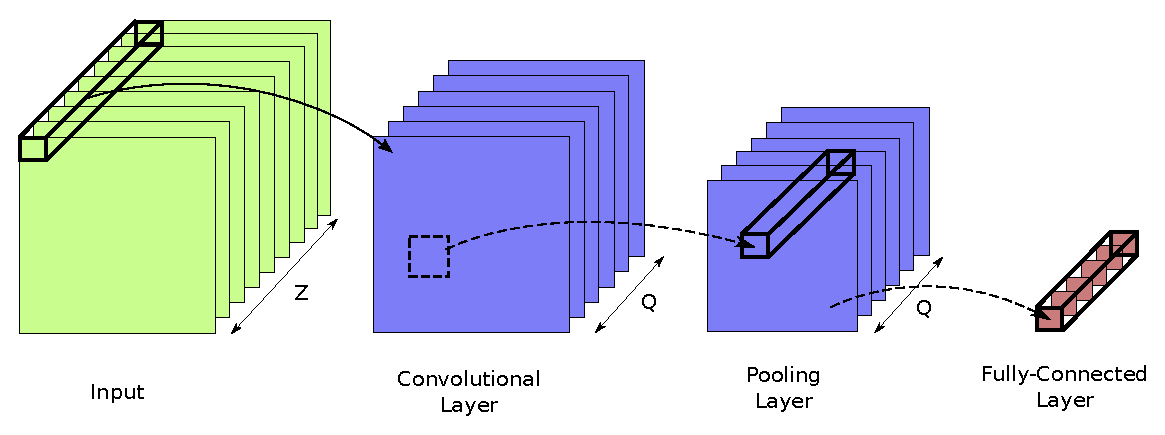
\includegraphics[width=.7\linewidth]{deep.eps}
\caption{Convolutional Neural Network Structure}
\label{fig:cnn}
\end{figure}


\begingroup
The convolutional layer uses different filters and computes the dot product between a small region in the previous layer and a set of weights. The output
of this calculation is usually described as an activation map. The computation for a single input layer and filter is shown in \autoref{fig:convlayer}.
The output for this filter is calculated through $1*1 + 1*1 = 2$. For multiple convolutional layers the activation maps are stacked on top of each other.
The number of filters is specified by $Q$ in \autoref{fig:cnn}. The input depth is defined by $Z$.
To control the output size of a convolutional layer depth, stride $S$ and zero-padding $P$ are used. Depth describes
the number of filters, which separately learn a different feature set. Stride specifies the number
of pixels a filter is moved. Zero-padding defines the padding used on the edges of input image. It is usually used to generate a
specific output. The output size of a convolutional layer is given by $(W - F + 2P)/S + 1$, where $W$ is the input
size and $F$ the filter size. If $S = 1$ zero-padding can be set to $P = (F - 1)/2$ to retain the input dimensions. Although this approach is only
presented for quadratic layers, $W$ and $F$ can be separately defined for each dimension.
\endgroup


\begin{figure}[ht]
\centering
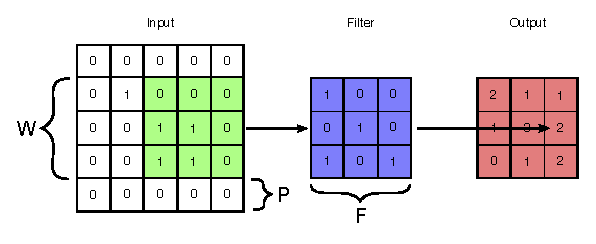
\includegraphics[width=.7\linewidth]{conv.eps}
\caption{Convolutional Layer Computation}
\label{fig:convlayer}
\end{figure}


\begingroup
Since convolutional layers usually add a lot of neurons to the model a pooling layer is applied to reduce the number of nodes.
The most common pooling layer simply finds the maximum value within a specified window and passes it on to the next layer.
This leads to a downsampling of the information in the current layer. Additonal fully-connected layers can be used to generate
a specific output volume \cite{ConvGit, ConvIntro, ConvVisual}.
\endgroup


\section{Autoencoders}\label{sec:section}

\begingroup
Autoencoders (AEs) are artificial neural networks used for efficient data encodings. These codes are found by creating
NNs that reproduce some input at the network's output. The structure of such a network is shown in \autoref{fig:autoencoder}.
The autoencoder is built using an encoding and decoding unit. The encoding unit compresses the input layer into
a lower-dimensional representation. The decoder of the autoencoder then uncompresses this code into a set of attributes
that closely matches the original input. This approach enables the network to ignore noisy input data. Another
advantage of autoencoders are non-existent data errors, since output and input are equivalent. Using other datasets might
introduce training errors into the model. In contrast, identity functions are easily verifiable.

After an autoencoder is trained each output usually has a unique latent representation in the network. This representation is
labelled as "Code" in \autoref{fig:autoencoder}. Apart from its compression characteristics, this code is used in
variational autoencoders (VAEs) to generate an output from a set of randomly chosen features \cite{VariationalAutoencoders}.
Furthermore, autoencoders can also be used to colorize and create higher resolution images. Both types
of autencoders are tested against adversarial attacks in this thesis.
\endgroup


\begin{figure}[ht]
\centering
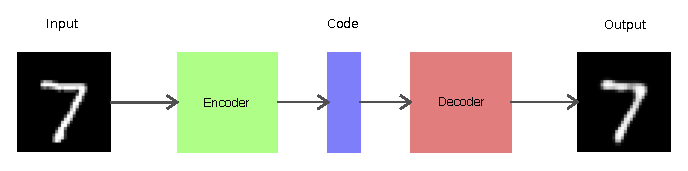
\includegraphics[width=.7\linewidth]{autoencoder.eps}
\caption{Autoencoder}
\label{fig:autoencoder}
\end{figure}

\begingroup
Instead of limiting the capacity of the network through its layers. It is possible to promote certain sets of features
through regularized autoencoders. For instance, sparse autoencoders are typically used to learn features for another
task such as classification. An autoencoder that has been regularized to be sparse must respond to unique features of
a dataset instead of acting as an identity function. Another class of regularized autoencoders are denoising autoencoders.
These networks attempt to remove noise that is added to an input image \cite{Denoise}.
\endgroup

\chapter{Adversarial Attacks}\label{sec:chapter}

\section{Introduction}\label{sec:section}

\begingroup
Misclassification of DNNs have become more prominent in recent years. Especially in
medical applications and automous driving errors of DNN can be fatal \cite{NeuralMed,ControlPipeline}.
To reduce the failure of these systems fast and secure methods to evaluate these networks are necessary.
In the following various optimization techniques are introduced to find networks prone to errors.
To compare different attack characteristics a regression problem is used.
Adversarial attacks (input perturbations for a NN) can be introduced into networks in many ways.
Eykholt et al. \cite{RealWorld} has shown that these attacks can be performed in the real world. The research paper
uses stickers and graffitis to test adversarial attacks.

Generally, the aim of an attacker is to create an additive perturbation $ \bm{\eta} \in \mathbb{R}^M$ with $M \triangleq n^{(1)}$ that is unnoticeable by
an outstanding entity. The loss or cost function for $\bm{x} + \bm{\eta}$ is given by $ \mcl{L}(\bm{x} + \bm{\eta}) = \lvert\lvert f(\bm{x} + \bm{\eta}) - \bm{y} \rvert\rvert^2_2 $.
The maximum input noise is limited through $\lvert\lvert \bm{\eta} \rvert\rvert_p \leq \epsilon$ with $\epsilon \in \mathbb{R}$ and $p \in \mathbb{N}$.
The objective of an attacker is to maximize this loss. Therefore, the problem can be defined as
\endgroup

\begin{equation}
\begin{aligned}
	\max_{ \bm{\eta} } \; \mcl{L}(\bm{x} + \bm{\eta}) = \max_{ \bm{\eta} } \; \lvert\lvert f(\bm{x} + \bm{\eta}) - \bm{y} \rvert\rvert^2_2 \quad s.t. \quad \lvert\lvert \bm{\eta} \rvert\rvert_p  \leq \epsilon \\
\end{aligned}
\label{intromax}
\end{equation}


\begingroup
Unfortunately, this problem cannot be easily solved, since $f(\bm{x}+\bm{\eta})$ depends on $\bm{\eta}$.
\endgroup


\section{Convex Attacks}\label{sec:section}

% Linear %
\subsection{Linear Programming Problem}\label{sec:section}

\begingroup
One of the earliest approaches to solve \ref{intromax} was the Fast Gradient Sign Method (FGSM), which was first introduced by Goodfellow et al. \cite{Goodfellow}. The paper
linearizes the cost function around $\bm{x}$ and sets $p=\infty$. The optimal max-norm is then given by
\endgroup

\begin{equation}
\begin{aligned}
	\bm{\eta} = \epsilon \; \text{sign}( \nabla_{\bm{x}} \mcl{L}) \quad w. \quad \lvert\lvert \bm{\eta} \rvert\rvert_{\infty} \leq \epsilon
\end{aligned}
\label{fastgradientsign}
\end{equation}

\begingroup
This linarization can be performed using a taylor expansion as shown in \ref{taylorlinear}. If $ \mcl{L}(\bm{x}) = \left\lvert\lvert f(\bm{x}) - \bm{y} \right\rvert\rvert^2_2 $
is used the product rule can be applied and the effect of $\bm{\eta}$ thoroughly studied.
\endgroup

\begin{equation}
\begin{aligned}
	\mcl{L}(\bm{x} + \bm{\eta}) &\approx \mcl{L}(\bm{x}) + \bm{\eta}^T \nabla \mcl{L}(\bm{x}) = \mcl{L}(\bm{x}) + \bm{\eta}^T \nabla \mcl{L}(\bm{x}) \\[10pt]
		&= \mcl{L}(\bm{x}) + \bm{\eta}^T \nabla( (\bm{y} - f(\bm{x}))^T (\bm{y} - f(\bm{x})) ) \\[10pt]
		&= \mcl{L}(\bm{x}) + \bm{\eta}^T \nabla( \bm{y}^T\bm{y} - f(\bm{x})^T \bm{y} + f(\bm{x})^T f(\bm{x}) - \bm{y}^T f(\bm{x}) ) \\[10pt]
		&= \mcl{L}(\bm{x}) + \bm{\eta}^T (-\bm{J}_f(\bm{x})^T \bm{y} - \bm{y}^T \bm{J}_f(\bm{x}) + \bm{J}_f(\bm{x}) f(\bm{x}) + f(\bm{x})^T \bm{J}_f(\bm{x})) \\[10pt]
		&= \mcl{L}(\bm{x}) - 2 \bm{\eta}^T \bm{J}_f(\bm{x}) ( \bm{y} - f(\bm{x}) ) \\
\end{aligned}
\label{taylorlinear}
\end{equation}

\begingroup
As shown above this leads to a problem for perfectly fitted models, where $ \bm{y} = f(\bm{x})$ because the gradient $\nabla \mcl{L} = 0$. This
is especially problematic for autoencoders, which add additonal features to the input like colorization. $\bm{y} \in \mathbb{R}^N$ is
usually unknown in these systems and needs to be determined during a first iteration of the DNN. Therefore,
another point $ \bm{\tilde{x}}$ needs be defined, which lies in close proximity to $\bm{x}$. In this point the gradient $ \nabla \mcl{L}(\bm{\tilde{x}}) \neq 0 $
and $ \lvert\lvert x - \tilde{x} \rvert\rvert_p \ll \epsilon $. Therefore, \ref{intromax} can now be generally solved through
\endgroup


\begin{equation}
% \tag{$\dagger$}
\begin{aligned}
	\max_{\bm{\eta}} \nabla \mcl{L}(\bm{\tilde{x}})^T \bm{\eta} \quad s.t. \quad \lvert\lvert \bm{\eta} \rvert\rvert_p \leq \epsilon
\end{aligned}
\label{maxlinopt}
\end{equation}

\begingroup
In the following, $\bm{\tilde{x}}$ and $\bm{x}$ are not further separated.
The closed-form solution for different $p$-norms are given below. Generally, a solution is found using
the upper boundary of the maximization problem.
\endgroup

\begin{equation}
\begin{aligned}
p = 1: & \quad \bm{\eta} = \epsilon \; \bm{e}_{k^\star} \quad w. \quad k^\star = \argmax_{k} \; \lvert (\nabla \mcl{L}(x))_k \rvert \\[20pt]
p = 2: & \quad \bm{\eta} = \epsilon \; \frac{\nabla \mcl{L}(\bm{x})}{\lvert\lvert \nabla \mcl{L}(\bm{x}) \rvert\rvert_2} \\[20pt]
p = \infty: & \quad \bm{\eta} = \epsilon \; \text{sign}(\nabla \mcl{L}(\bm{x}))
\end{aligned}
\label{linear_programming_closed}
\end{equation}


$\bm{Proof.}$ The proof for all linear solutions follows the Hölder inequality \cite{Hoelder}. The theorem states that if $q \triangleq \frac{p}{p-1}$ and $p, q \in [1, \infty]$
the upper boundary can be found by

\begin{equation}
\begin{aligned}
	\lvert\lvert \bm{f}^T\bm{g} \rvert\rvert_1 \leq \lvert\lvert \bm{f} \rvert\rvert_p \lvert\lvert \bm{g} \rvert\rvert_q
\end{aligned}
\label{hoelders_inequality}
\end{equation}

and can be reached through

\begin{equation}
\begin{aligned}
	\sup_{\lvert\lvert \bm{\eta} \rvert\rvert_p \leq 1} \nabla \mcl{L}(\bm{x})^T \bm{\eta} = \lvert\lvert \nabla \mcl{L}(\bm{x}) \rvert\rvert_q
\end{aligned}
\label{linear_programming_sup}
\end{equation}

The upper bound is then reached through

\begin{equation}
\begin{aligned}
	\bm{\eta} = - \epsilon \frac{1}{\lvert\lvert \nabla \mcl{L}(\bm{x}) \rvert\rvert_q^{q-1}} \cdot ( \text{sign}( \nabla \mcl{L}(\bm{x}) ) \odot \lvert \nabla \mcl{L}(\bm{x}) \rvert^{q-1} )
\end{aligned}
\label{linear_programming_solution}
\end{equation}

Since there is no larger supremum, $\bm{\eta}$ needs to be the optimal solution.
Setting $p$ to the respective norm then results in the closed-form solutions in \ref{linear_programming_closed}. $ \blacksquare $

\begingroup
To find even more accurate solutions to the linear programming problem iterative solutions can be used. One of the first attempts was the
DeepFool algorithm \cite{DeepFool}. After calculating an adversarial example for a particular input vector, a new noise vector is calculated
using the previous adversarial input. For example, the iterative solution for the $l_{\infty}$-norm
is calculated using the following pseudocode. Iterative solutions for other norms follow the same procedure.
\endgroup

%%% PSEUDO CODE

\begin{algorithm}
\caption{Iterative Solution for $p = \infty$ (Linear Programming Problem)}
\label{alg:euclid}
\begin{algorithmic}[1]
\State \textbf{input:} $\; \bm{x}, f(\bm{x}), \bm{\eta}, N$
\State \textbf{output:} $\; \bm{\eta}$
\State \textbf{initialize:} $\bm{\tilde{x}} \gets \bm{x}$
\For{$i \gets 1, ..., N$}
	\State $ \bm{\eta} \gets \frac{\bm{\epsilon}}{N} \; \text{sign}(\nabla \mcl{L}(\bm{\tilde{x}})) $
	\State $ \bm{\tilde{x}} \gets \bm{\tilde{x}} + \bm{\eta} $
\EndFor
\end{algorithmic}
\end{algorithm}


% Quadratic %

\subsection{Quadratic Programming Problem}\label{sec:section}


Similar to the loss function,
$ f(\bm{x}) $ can be generally regarded as a non-convex and non-linear function. But since $ \lvert\lvert \bm{\eta} \rvert\rvert_p \leq \epsilon $,
the function can be approximated using a taylor expansion in close proximity to $\bm{x}$. This results in the following
quadratic programming problem.


\begin{equation}
\begin{aligned}
\mcl{L}(\bm{x} + \bm{\eta}) &= \lvert\lvert \bm{y} - f(\bm{x} + \bm{\eta}) \rvert\rvert^2_2 \\[10pt]
&= (\bm{y} - f(\bm{x} + \bm{\eta}))^T(\bm{y} - f(\bm{x} + \bm{\eta})) \\[10pt]
&= \bm{y}^T\bm{y} - f(\bm{x} + \bm{\eta})^T\bm{y} - \bm{y}^T f(\bm{x} + \bm{\eta}) + f(\bm{x} + \bm{\eta})^Tf(\bm{x} + \bm{\eta}) \\[10pt]
&= \lvert\lvert \bm{y} \rvert\rvert^2_2 - 2 \bm{y}^T f(\bm{x} + \bm{\eta}) + \lvert\lvert f(\bm{x} + \bm{\eta}) \rvert\rvert^2_2 \\[10pt]
&\approx \lvert\lvert \bm{y} \rvert\rvert^2_2 - 2 \bm{y}^T (f(\bm{x}) + \bm{J}_f(\bm{x})\bm{\eta}) + \lvert\lvert f(\bm{x}) + \bm{J}_f(\bm{x}) \bm{\eta} \rvert\rvert^2_2 \\[10pt]
&= \lvert\lvert \bm{y} \rvert\rvert^2_2 - 2 \bm{y}^T (f(\bm{x}) + \bm{J}_f(\bm{x})\bm{\eta}) + (f(\bm{x}) + \bm{J}_f(\bm{x})\bm{\eta})^T(f(\bm{x}) + \bm{J}_f(\bm{x})\bm{\eta}) \\[10pt]
&= \cancel{ \lvert\lvert \bm{y} \rvert\rvert^2_2 } - 2 \bm{y}^T ( \cancel{ f(\bm{x}) } + \bm{J}_f(\bm{x})\bm{\eta})) + \cancel{  \lvert\lvert f(\bm{x}) \rvert\rvert^2_2 } + 2 \bm{\eta}^T \bm{J}_f(\bm{x})^Tf(\bm{x}) + \lvert\lvert \bm{J}_f(\bm{x}+\bm{\eta}) \rvert\rvert^2_2 \\[10pt]
&= 2 \bm{\eta}^T \bm{J}_f(\bm{x})^T (f(\bm{x}) - \bm{y}) + \lvert\lvert \bm{J}_f(\bm{x}) \bm{\eta} \rvert\rvert^2_2 \\
\end{aligned}
\label{taylorquadratic}
\end{equation}

\begingroup
The simplified convex problem for $\mcl{L}$ is further simplified by using $\bm{y} \approx f(\bm{x})$.
Therefore, the problem gets simpliefied to the following form.
\endgroup

\begin{equation}
\begin{aligned}
	\max_{\bm{\eta}} \; \lvert\lvert \bm{J}_f(\bm{x}) \bm{\eta} \rvert\rvert_2^2 \quad s.t. \quad \lvert\lvert \bm{\eta} \rvert\rvert_p \leq \epsilon
\end{aligned}
\label{quadintro}
\end{equation}

\begingroup
This problem leads to a convex quadratic bowl maximization under a $l_p$-ball constraint. The maximization problem \ref{quadintro} can be reformulated using
\endgroup

\begin{equation}
\begin{aligned}
	\lvert\lvert \bm{J}_f(\bm{x}) \bm{\eta} \rvert\rvert_2 = \epsilon \; \lvert\lvert \bm{J}_f(\bm{x}) \frac{\bm{\eta}}{\epsilon} \rvert\rvert_2
\end{aligned}
\label{quadfollow}
\end{equation}

\begingroup
Due to $\lvert\lvert \frac{\bm{\eta}}{\epsilon} \rvert\rvert_p \leq 1$, the problem can be solved using operator norms. If
$\bm{M}: V \rightarrow W$ is a linear transformation the operator norm is given by the subsequent term.
\endgroup

\begin{equation}
\begin{aligned}
	\lvert\lvert \bm{M} \rvert\rvert_{V \rightarrow W} = \sup_{\bm{v} \in V \backslash \{0\}} \frac{\lvert\lvert \bm{M v} \rvert\rvert_W}{\lvert\lvert \bm{v} \rvert\rvert_V} = \sup_{\lvert\lvert \bm{v} \rvert\rvert_V \leq 1} \lvert\lvert \bm{M v}  \rvert\rvert_W
\end{aligned}
\label{operatornorm}
\end{equation}

\begingroup
Since $\lvert\lvert \bm{\eta} \rvert\rvert_p = \epsilon$ is the upper bound, \ref{quadfollow} can be estimated through $\epsilon \; \lvert\lvert \bm{J}_f(\bm{x}) \frac{\bm{\eta}}{\epsilon} \rvert\rvert_2 \leq \epsilon \; \lvert\lvert \bm{J}_f(\bm{x}) \rvert\rvert_{p \rightarrow 2}$.
For $l_1$ and $l_2$ this operator norm has a closed-form solution.

For $l_2$ a solution is provided by a theorem from Ky Fan, 1950 \cite{KyFan, BigData}. If $\bm{M} \in \mathbb{R}^{n \times n}$ is a symmetric matrix with sorted
eigenvalues $\lambda_n (\bm{M}) \leq ... \leq \lambda_1 (\bm{M})$ and $\bm{v} \in \mathbb{R}^n$ a vector. The solution is given by
\endgroup

%% kyfan theorem l2 optimization

\begin{equation}
\begin{aligned}
	\max_{\lvert\lvert \bm{v} \rvert\rvert = 1, \bm{v} \in \mathbb{R}^n} \bm{v^T M v} = \lambda_{max} (\bm{M})
\end{aligned}
\label{kyfanmax}
\end{equation}


\begingroup
Therefore, to maximize \ref{quadfollow} the eigenvector $\bm{v}_{max}$ of $\bm{J}_f(\bm{x})^T \bm{J}_f(\bm{x})$ needs to be found, which corresponds to
the largest eigenvalue. Then, the optimal solution to \ref{quadintro} is given by $\bm{\eta} = \pm \epsilon \; \bm{v}_{max}$ \cite{BigData}.
\endgroup


%%%% PROOF KY FAN

\begingroup
$\bm{Proof.}$ Suppose that $\bm{u}_1, ..., \bm{u}_n$ are eigenvectors of $\bm{M}$ corresponding to $\lambda_1(\bm{M}) \geq ... \geq \lambda_n(\bm{M})$
and $\bm{U} = [\bm{u}_1, ..., \bm{u}_n]$. Every vector $\bm{v}$ can be written as $\bm{v} = a_1 \bm{u}_1 + ... + a_n \bm{u}_n = \bm{U} \bm{a}$ where
$\bm{a} = [a_1, ..., a_n]^T$. We get to
\endgroup

\begin{equation}
\begin{aligned}
	\max_{\bm{v} \in \mathbb{R}^n, \bm{v}^T\bm{v}=1} \bm{v}^T \bm{M} \bm{v} &= \max_{\bm{a} \in \mathbb{R}^n, \bm{a}^T\bm{a}=1} \bm{a}^T\bm{U}^T \bm{M} \bm{U}\bm{a} \\
	&=  \max_{\bm{a} \in \mathbb{R}^n, \bm{a}^T\bm{a}=1} \sum_{i=1}^n \lambda_i (\bm{M}) a_i^2 \leq \lambda_1 (\bm{M})
\end{aligned}
\label{kyfan_proof}
\end{equation}

$\blacksquare$

%% l1 closed-form solution

\begingroup
For $p = 1$ a closed-form solution is provided by \ref{l1_norm_solution}. It can be assumed that the conditions from \ref{operatornorm} still apply.
\endgroup

\begin{equation}
\begin{aligned}
	\lvert\lvert \bm{M} \rvert\rvert_{1 \rightarrow 2} = \max_{k \in \{1, ..., n\}} \lvert\lvert \bm{m}_k \rvert\rvert_2
\end{aligned}
\label{l1_norm_solution}
\end{equation}

\begingroup
$\bm{m}_k$ defines the $k$-th column vector of the matrix $\bm{M}$. This closed-form solution leads to
\endgroup

\begin{equation}
\begin{aligned}
	\epsilon \; \lvert\lvert \bm{J}_f(\bm{x}) \rvert\rvert_{1 \rightarrow 2} \leq \max_{k \in \{1, ..., n\}} \lvert\lvert \bm{J}_f(\bm{x})_k \rvert\rvert_2
\end{aligned}
\label{l1solution}
\end{equation}

\begingroup
and
\endgroup

\begin{equation}
\begin{aligned}
	\bm{\eta} = \pm \epsilon \; \bm{e}_{k} \quad s.t. \quad k = \argmax_{k \in \{1, ..., n\}} \lvert\lvert \bm{J}_f(\bm{x}) \rvert\rvert_2
\end{aligned}
\label{l1final}
\end{equation}


%%%%% Proof l1
$\bm{Proof.}$ It can be assumed that $\lvert\lvert \bm{v} \rvert\rvert_1 \leq 1$ and $\bm{M} \in \mathbb{R}^{n \times n}$. The column with
the largest norm $\lvert\lvert \bm{m}_k \rvert\rvert_2$ is defined as $\bm{m}_{\alpha}$ with the corresponding scalar $\alpha$. The
proof now follows an iterative procedure of finding an additonal column $\bm{m}_{\beta}$ that improves the solution.


\begin{equation}
\begin{aligned}
	\lvert\lvert \bm{M v} \rvert\rvert_2^2 &= \lvert\lvert \alpha \bm{m}_{\alpha} + \beta \bm{m}_{\beta} \rvert\rvert_2^2
	&\leq \alpha^2 \lvert\lvert \bm{m}_{\alpha} \rvert\rvert_2^2 + \beta^2 \lvert\lvert \bm{m}_{\beta} \rvert\rvert_2^2 \leq \lvert\lvert \bm{m}_{\alpha} \rvert\rvert_2^2
\end{aligned}
\label{l1_proof}
\end{equation}

$\blacksquare$

\begingroup
Intuitively, $\bm{\eta}$ needs to point into the same direction of the maximum of $\bm{J}_f(\bm{x})$ to optimally solve the maximization problem.
For the quadratic programming problem, the closed-form solutions are provided below in a compact form. For $p = \infty$
the problem is unfornuately NP-hard and can therefore not be solved without iterating through all the possible combinations. An
overview of solutions to an operator norm problem is given by \autoref{operatorcompu}.
\endgroup

\begin{equation}
\begin{aligned}
p = 1: \quad &\bm{\eta} = \pm \epsilon \; \bm{e}_{k} \quad s.t. \quad k = \argmax_{k \in \{1, ..., n\}} \lvert\lvert \bm{J}_f(\bm{x}) \rvert\rvert_2 \\[20pt]
p = 2: \quad &\bm{\eta} = \pm \epsilon \; \bm{v}_{max}
\end{aligned}
\label{quadraticclosedform}
\end{equation}

\begin{table}[]
\centering
\def\arraystretch{1.5}
\begin{tabular}{|c|c|c|c|c|}
\hline
                                 & \multicolumn{4}{c|}{\textbf{Co-Domain}}                                                                                                                                                                                       \\ \hline
                                 &      & $l_1$                                                                    & $l_2$                                                                    & $l_\infty$                                                       \\ \hline
 															 	 & $l_1$   & \begin{tabular}[c]{@{}c@{}}Maximum $l_1$-norm\\ of a column\end{tabular} & \begin{tabular}[c]{@{}c@{}}Maximum $l_2$-norm\\ of a column\end{tabular} & \begin{tabular}[c]{@{}c@{}}Maximum $l_\infty$-norm\\ of a column\end{tabular} \\ \cline{2-5}
\multirow{1}{*}{\textbf{Domain}} & $l_2$   & NP-hard                                                               & \begin{tabular}[c]{@{}c@{}}Maximum singular\\ value\end{tabular}      & \begin{tabular}[c]{@{}c@{}}Maximum $l_2$-norm\\ of a row\end{tabular}      \\ \cline{2-5}
                                 & $l_\infty$ & NP-hard                                                            & NP-hard                                                               & \begin{tabular}[c]{@{}c@{}}Maximum $l_1$-norm\\ of a row\end{tabular}      \\ \hline
\end{tabular}

\caption{Operator Norm Computability}
\label{operatorcompu}

\end{table}

%% Single Pixel attacks %%

\section{Single Subset Attacks}\label{sec:section}

\begingroup
Single Pixel Attacks like \cite{SingleClassification} have proven to be successful in fooling various DNNs
for classification tasks. The attacker's goal in this scenario is to find a single pixel, which can be modified,
to create a highly disturbed output. The definition of this attack varies in various research
papers. For instance, Su et al. \cite{SingleClassification} suggests to modifiy only one color channel and to set
other dimensions to zero. In the following, we will attempt to generalize this approach using a greedy approach. The entire
set of pixel information $\mcl{M} = \{1, ..., M\}$ can be devided into $\mcl{S} = \{\mcl{S}_1, ..., \mcl{S}_S\}$
subsets. Each subset represents the color channels from one pixel. The size is determined through $Z = \frac{M}{S}$. Pixels in
a subset are described using $\mcl{S}_S = \{i^1_S, ..., i^Z_S\}$. To count the number of changed subsets, the
$\lvert\lvert \; \cdot \; \rvert\rvert_{0, \mcl{S}}$ zero-$\mcl{S}$ norm is introduced. For $\lvert\lvert \bm{\eta} \rvert\rvert_{0, \mcl{S}}$ this norm counts the number of modified channels.
If an attacker only attempts to change a single pixel the problem can be formulated in the following way:
\endgroup

\begin{equation}
\begin{aligned}
	\max_{\bm{\eta}} \mcl{L}(\bm{x} + \bm{\eta}) \quad s.t. \quad \lvert\lvert \bm{\eta} \rvert\rvert_{\infty} \leq \epsilon \;, \; \lvert\lvert \bm{\eta} \rvert\rvert_{0, \mcl{S}} = 1
\end{aligned}
\label{singlesubsetgeneral}
\end{equation}


\subsection{Single Subset Attack for the Linear Problem}\label{06_single_linear}

\begingroup
As shown in \ref{maxlinopt} the maximization problem in \ref{singlesubsetgeneral} can be approximated using a taylor expansion. The
resulting linear programming problem is shown in \ref{singlesubsetlinear}. Since only one subset is supposed to be modified the
problem can be rewritten as \ref{singlesubsetrewrite}.
\endgroup

\begin{equation}
\begin{aligned}
	\max_{\bm{\eta}} \nabla \mcl{L}(\bm{x})^T \bm{\eta} \quad s.t. \quad \lvert\lvert \bm{\eta} \rvert\rvert_{\infty} \leq \epsilon \;, \; \lvert\lvert \bm{\eta} \rvert\rvert_{0, \mcl{S}} = 1
\end{aligned}
\label{singlesubsetlinear}
\end{equation}

\begin{equation}
\begin{aligned}
	\bm{\eta_{s}} = \argmax_{\bm{\eta}} \nabla \mcl{L}(\bm{x})^T \bm{\eta} \quad s.t. \quad \lvert\lvert \bm{\eta} \rvert\rvert_{\infty} \leq \epsilon \;, \; (\bm{\eta})_{i_s^z} = 0 \; \forall i_s^z \not\in \mcl{S}_{\mcl{S}}
\end{aligned}
\label{singlesubsetrewrite}
\end{equation}

\begingroup
This problem is maximized by choosing a subset for $\bm{\eta}$ that has the largest norm $\lvert\lvert \nabla \mcl{L}(\bm{x}) \rvert\rvert_{\infty} $.
Afterwards, $\bm{\eta}$ is determined by the direction of $\nabla \mcl{L}(\bm{x})$ in the chosen subset. The problem is further constrained by
$\lvert\lvert \bm{\eta} \rvert\rvert_{\infty} \leq \epsilon$. Therefore, the optimal solution lies on the edges of
the hypercube $\lvert\lvert \bm{\eta} \rvert\rvert_{\infty} = \epsilon$. This geometric interpretation leads to the following closed-form solution.
\endgroup


\begin{equation}
\begin{aligned}
	\bm{\eta^{*}} = \bm{\eta_{s^*}} \quad w. \quad s^{*} = \argmax_s \sum_{z=1}^{Z} \lvert \nabla (\mcl{L}(\bm{x}))_{i^z_s} \rvert \; , \; \bm{\eta}_s = \epsilon \sum^{Z}_{z=1} \text{sign}((\nabla \mcl{L}(\bm{x}))_{i_s^z}) \bm{e}_{i^z_s}
\end{aligned}
\label{singlelinearsolution}
\end{equation}

\begingroup
$\bm{\eta_s}$ determines the optimal subset perturbation. A single subset is then selected based on the maximum change to the cost function $\mcl{L}$.
The pseudocode for the linear subset attack is provided by Algorithm 2. For multiple pixels the routine can be run iteratively with $\bm{P}$
holding all used pixels after each iteration.
\endgroup


\begin{algorithm}[ht]
\caption{Single Subset Attack (Linear Solution)}
\label{alg:single_linear}
\begin{algorithmic}[1]
\State \textbf{input:} $h_{opt}, w_{opt}, \theta$
\State \textbf{output:} $\bm{P}, \bm{\eta}_{opt}$
\For{$h \gets 1, ..., H$}
	\For{$w \gets 1, ..., W$}
		\State $\phi_s \gets \sum_{z=1}^Z \lvert \nabla \mcl{L}_{i_s^z} \rvert$
		\If{$\phi_s > \theta \; and \; (h, w) \not\in \bm{P}$}
			\State $h_{opt}, w_{opt}, \bm{\eta}_{opt} \gets h, w, \epsilon \cdot \text{sign}(\nabla \mcl{L}_s)$
			\State $\theta \gets \phi_s$
		\EndIf
	\EndFor
\EndFor
\State $\bm{P} \gets (h_{opt}, w_{opt})$
\end{algorithmic}
\end{algorithm}


\subsection{Single Subset Attack for the Quadratic Problem}\label{06_single_quadratic}


\begingroup
In the same manner as described in \autoref{06_single_linear}, a solution can be found for the quadratic problem.
First of all, the initial problem \ref{06_single_quadratic_problem} is simplified by fixing the subset modified by an attacker
again to $\bm{\eta}_s$.
\endgroup


\begin{equation}
\begin{aligned}
	\max_{\bm{\eta}} \lvert\lvert \bm{J}_f(\bm{x}) \bm{\eta} \rvert\rvert_2^2 \quad s.t. \quad \lvert\lvert \bm{\eta} \rvert\rvert_{\infty} \leq \epsilon \; , \; \lvert\lvert \bm{\eta} \rvert\rvert_{0,\mcl{S}} = 1
\end{aligned}
\label{06_single_quadratic_problem}
\end{equation}

\begin{equation}
\begin{aligned}
	\bm{\eta}_s = \argmax_{\eta} \lvert\lvert \bm{J}_f(\bm{x}) \bm{\eta} \rvert\rvert_2^2 \quad s.t. \quad \lvert\lvert \bm{\eta} \rvert\rvert_{\infty} \leq \epsilon \;, \; (\bm{\eta})_{i_s^z} = 0 \; \forall i_s^z \not\in \mcl{S}_{\mcl{S}}
\end{aligned}
\label{06_single_quadratic_problem_rewrite}
\end{equation}

\begingroup
In contrast to the linear subset attack, there is not a closed-form solution for the quadratic problem.
Instead it is possible to reduce the complexity by finding a suboptimal solution.

Geometrically, \ref{06_single_quadratic_problem_rewrite} can be viewed
as the maximization of a quadratic bowl over a hypercube. By limiting the solution space, we get $\bm{\eta}_s = \epsilon \sum_{z=1}^{Z} \rho_{i_s^z}^* \bm{e}_{i^z_s}$
with $\bm{\rho^*_s} = (\rho_{i_s^1}, ..., \rho_{i_s^z})^T \in \{ -1, +1\}^Z $. Therefore, foreach subset the problem gets rewritten to \ref{06_single_quadratic_solution_rho_1} and \ref{06_single_quadratic_solution_rho_2}.
\endgroup

\begin{equation}
\begin{aligned}
	\bm{\eta}^* = \bm{\eta}_{s*} \quad w. \quad s^* = \argmax_s \lvert\lvert \bm{J}_f(\bm{x}) \bm{\eta}_s \rvert\rvert_2^2 \; , \; \bm{\eta}_s = \epsilon \sum_{z=1}^{Z} \rho_{i_s^z}^* \bm{e}_{i^z_s}
\end{aligned}
\label{06_single_quadratic_solution_rho_1}
\end{equation}

\begin{equation}
\begin{aligned}
	\bm{\rho}_s^* = \argmax_{\rho_s \in \{-1, +1\}^z} \lvert\lvert \bm{J}_f(\bm{x})(\epsilon \sum_{z=1}^{Z} \rho_{i_s^z} \bm{e}_{i_s^z}) \rvert\rvert_2^2 = \argmax_{\bm{\rho}_s \in \{-1, +1\}^Z} \sum_{z=1}^Z \sum_{w=1}^Z \rho_{i_s^z} \rho_{i_s^w} \bm{J}_{i_s^z}^T \bm{J}_{i_s^w}
\end{aligned}
\label{06_single_quadratic_solution_rho_2}
\end{equation}

\begingroup
To find a solution to this NP-hard problem, $\bm{\eta}_s^*$ can be approximated using a greedy method. This is achieved by sorting $\lvert\lvert \bm{J}_{i_s^1} \rvert\rvert_2 \geq ... \geq \lvert\lvert \bm{J}_{i_s^z} \rvert\rvert_2$ and setting $\bm{\rho}_{i_s^1}^* = 1$.
Afterwards, all $\rho_{i_s^z}^*$ are calculated recursively in \ref{06_single_quadratic_recursive} using $\rho_{i_1^s}^*$ as a starting point.
\endgroup

\begin{equation}
\begin{aligned}
	\rho_{i_s^z}^* = \text{sign}((\sum_{j=1}^{z-1} \rho_{i_s^j}^* \bm{J}_{i_s^z})^T \bm{J}_{i_s^z}) \quad \forall z = 2, ..., Z
\end{aligned}
\label{06_single_quadratic_recursive}
\end{equation}


\begingroup
The entire iterative procedure is similar to the solution of Goemans and Williamson to the MacCut problem \cite{MaxCut}. Therefore, the given solution is also limited by the same approximation factor $R = 0.87856$ with $\lvert ALG \rvert \geq R \cdot \lvert OPT \rvert$.
For an image with three color channels ($Z=3$), $\rho_{i_s^z}^*$ looks the following way.
\endgroup

\begin{equation}
\begin{aligned}
z = 1: \quad & \rho_{i_s^1}^* = 1 \\[10pt]
z = 2: \quad & \rho_{i_s^2}^* = \text{sign}( (\rho_{i_s^1}^* \bm{J}_{i_s^1})^T \bm{J}_{i_s^2} ) \\[10pt]
z = 3: \quad & \rho_{i_s^3}^* = \text{sign}( (\rho_{i_s^1}^* \bm{J}_{i_s^1} + \rho_{i_s^2}^* \bm{J}_{i_s^2})^T \bm{J}_{i_s^3} ) \\[10pt]
\end{aligned}
\label{rho_example_z_3}
\end{equation}


\begin{algorithm}[ht]

\caption{Single Subset Attack (Quadratic Solution)}
\label{alg:single_quadratic}
\begin{algorithmic}[1]
\State $\bm{P}, \bm{J}_{norm} \gets None, 0$
\For{$h \gets 1, ..., H$}
	\For{$w \gets 1, ..., W$}
		\For{$d \gets 1, ..., D$}
			\State $n_d \gets \lvert\lvert \bm{J}_{i_s^d} \rvert\rvert_2$
		\EndFor
		\State $\rho_{i_s^1}^*, \hat{\bm{J}}, \bm{I} \gets 1, \bm{J}_{i_s^1}, reverse(argsort(n_1, ..., n_D))$
		\If{$D > 0$}
			\For{$k \gets 2, ..., D$}
				\State $\rho_{i_s^k}^* \gets \text{sign}( (\sum_{j=1}^{k-1} \rho_{i_s^{\bm{I}_k}}^* \bm{J}_{i_s^j})^T \bm{J}_{i_s^{\bm{I}_k}} )$
				\State $\hat{\bm{J}} \gets \hat{\bm{J}} + \rho_{i_s^{\bm{I}_k}}^* \cdot \bm{J}_{i_s^{\bm{I}_k}}$
			\EndFor
		\EndIf
		\If{$\lvert\lvert \sum_{j=1}^{k} \rho_{i_s^k}^* \bm{J}_{i_s^j} \rvert\rvert_2 > \bm{J}_{norm}$ and $(h, w) \not\in \bm{P}$}
			\State $h_{opt}, w_{opt}, \rho_{opt} \gets h, w, \rho^*$
			\State $\bm{J}_{norm} \gets \lvert\lvert \sum_{j=1}^{k} \rho_{i_s^k}^* \bm{J}_{i_s^j} \rvert\rvert_2$
		\EndIf
	\EndFor
\EndFor
\State $\bm{P}, \bm{\eta}_s^* \gets (h_{opt}, w_{opt}), \epsilon \cdot \rho_{opt}$

\end{algorithmic}
\end{algorithm}

\chapter{Simulation Results}\label{sec:chapter}

\section{Simulation Setup}\label{sec:section}

\begingroup
To model different adversarial attacks we mainly rely on Python 3.6 \cite{Python} and Tensorflow 1.7 \cite{Tensorflow}.
Tensorflow is a math library used for machine learning applications such as neural networks. The framework makes
it easy to develop DNNs with more than one hidden layer. This is especially helpful for more complex DNN architectures.
Furthermore, tensorflow provides a lot of necessary algorithms for backpropagation out-of-the-box. Therefore, the
development time gets heavily reduced.

The project itself is structured in a modular form. The datasets object enables access to the CIFAR, MNIST, SET14
and STL10 dataset. CIFAR (32x32) was published by the Canadian Institute for Advanced Research and is mainly used for object
classification. MNIST (28x28) contains a database of handwritten digits in black and white. It is one of the most
basic datasets, primarily used for character recognition. STL10 is a higher resolution (96x96)
object classification dataset. SET14 contains a selected set of popular test images.
Models used in this project are defined in the $models.json$ file. Adversarial examples are
generated in the $adversarial.py$ file. Norms and models can be selected using commands specified in the parser object. Final
results are saved in $csv$ and $eps$ files stored in the $results$ folder.
\endgroup

\begingroup
To test the effectiveness of adversarial attacks presented in previous sections, various models and datasets are used.
For comparibility reasons, the focus was set on autoencoders reproducing an identity function. Furthermore, attacks
were tested against convolutional AEs like colorization or super-resolution models.
An overview of the models and datasets used in the simulations is provided
by \autoref{ModelTable}.

FCNN is a fully-connected model, which is trained based on grayscale images of the MNIST dataset. The trained network
has a compression rate of 96\%. FCNN2 is similarly trained for the MNIST dataset, but uses convolutional layer with
a fully-connected layer in the center of the ntwork. For CIFAR, FCNN3 is trained as a fully-connected network with a
compression rate of 50\%. As an activation function all layers in the FCNN networks except the output layer use ReLu.
The output is provided using a Sigmoid function. ReLu offers better convergence properties than formerly used
TanH or Sigmoid functions. This is due to the higher linearity of the ReLu function.
The training of all the FCNN models was performed using an Adam Optimizer with a decreasing learning
rate $\alpha$.

AEN\_STL10 relies entirely on convolutional layers. The same holds true for KOALA \cite{KoalaModel} and C\_DCSCN
\cite{SuperModel}. Each convolutional layer in both models uses a ReLu activation function. For the super-resolution
model LeakyReLu is used to avoid the "dying ReLu" problem. Outputs of these
autoencoders are transformed to be plotted in RGB afterwards. For instance, the KOALA model requires the CbCr channel
to be merged with the Y color channel.

C\_DCSCN is trained to return an upsampled version of an input image. The underlying model first uses a bicubic interpolation
to approximate the super-resolution image. Afterwards, a residual CNN is created that focusses on learning the
residual between the original image and bicubic interpolation of the low resolution and high resolution
image \cite{SuperModel,SuperModel2}. An overview of the structure of the C\_DCSCN model is given by \autoref{c_dcscn_network_structure}.
Training of C\_DCSCN was performed using dropout. This technique removes a certain
portion (dropout rate) of nodes during training. This avoids training only a small set of the topology for the actual
classification or regression problem.
\endgroup


\begin{table}[]
\centering
\def\arraystretch{1.8}
\caption{Models and Datasets}
\label{ModelTable}
\begin{tabular}{|c|c|c|c|c|}
\hline
\textbf{Model} & \textbf{Dataset} & \textbf{Description} & \textbf{Input} & \textbf{Output} \\ \hline
FCNN           & MNIST            & Autoencoder          & Y              & Y               \\ \hline
FCNN2          & MNIST            & Autoencoder          & Y              & Y               \\ \hline
FCNN3          & CIFAR            & Autoencoder          & RGB            & RGB             \\ \hline
AEN\_STL10     & STL10            & Autoencoder          & RGB            & RGB             \\ \hline
KOALA          & STL10            & Colorization         & Y              & CbCr            \\ \hline
C\_DCSCN       & SET14            & Super-Resolution     & Y              & Y               \\ \hline
\end{tabular}
\end{table}


\begin{figure}[ht] % "[t!]" placement specifier just for this example
	\centering
\includegraphics[width=.7\linewidth]{\detokenize{c_dcscn_network_structure}}
\caption{C\_DCSCN structure as shown in \cite{SuperModel}}
\label{c_dcscn_network_structure}
\end{figure}



\begingroup
The Peak Signal-To-Noise Ratio (PSNR) describes the ratio between the maximum possible signal power and the power of the noise.
Most commonly the ratio is defined by \ref{07_psnr_definition} and \ref{07_mse_definition} \cite{PSNRConversion}. In these equations MAX defines
the maximum pixel value, $N$ the amount of given pixels and channels and $\hat{x}$ the noisy image itself.
\endgroup

\begin{equation}
\begin{aligned}
	\text{PSNR} = 10 \cdot log_{10} (\frac{\text{MAX}^2}{\text{MSE}})
\end{aligned}
\label{07_psnr_definition}
\end{equation}

\begin{equation}
\begin{aligned}
	\text{MSE} = \frac{1}{N} \sum_{i=1}^N (\hat{x}_i - x_i)^2
\end{aligned}
\label{07_mse_definition}
\end{equation}

\begingroup
Unfortunately, the input perturbation is limited by the $p$-norm $\lvert\lvert \bm{\eta} \rvert\rvert_p \leq \epsilon$ and only
$\epsilon$ is given. Therefore, the upper boundary needs to be found in terms of the $l_2$-norm.
\endgroup

\begin{equation}
\begin{aligned}
p=1: \quad & \lvert\lvert \bm{\eta} \rvert\rvert_{1 \rightarrow 2} \leq \epsilon \\[10pt]
p=2: \quad & \lvert\lvert \bm{\eta} \rvert\rvert_{2 \rightarrow 2} \leq \epsilon \\[10pt]
p=\infty: \quad & \lvert\lvert \bm{\eta} \rvert\rvert_{\infty \rightarrow 2} \leq \epsilon^2 N
\end{aligned}
\label{operator_epsilon}
\end{equation}

\begingroup
Using these approximations and setting $\text{MAX} = 1$ leads to the following PSNRs.
\endgroup

\begin{equation}
\begin{aligned}
p=1: \quad & \text{PSNR} = 10 \cdot log_{10} (\frac{N}{\epsilon}) \\[10pt]
p=2: \quad & \text{PSNR} = 10 \cdot log_{10} (\frac{N}{\epsilon}) \\[10pt]
p=\infty: \quad & \text{PSNR} = 10 \cdot log_{10} (\frac{N}{\epsilon^2}) = -20 \cdot log_{10} (\epsilon)
\end{aligned}
\label{psnr_simplify}
\end{equation}

\begingroup
Super-resolution and colorization models sometimes do not stay within the same color spaces. To convert between
the YCbCr and RGB color space the following conversion is necessary \cite{YCbCrConversion}. RGB values follow
through the inverse.
\endgroup

\begin{equation}
\begin{bmatrix}
Y \\
Cb \\
Cr
\end{bmatrix}
=
\begin{bmatrix}
0 \\
128 \\
128
\end{bmatrix}
+
\begin{bmatrix}
0.299 & 0.587 & 0.114 \\
-0.168736 & -0.331264 & 0.5 \\
0.5 & -0.41868 & -0.081312
\end{bmatrix}
\begin{bmatrix}
R \\
G \\
B
\end{bmatrix}
\end{equation}

\section{Results}\label{sec:section}

\begingroup
All the test results, which were observed during this thesis, can be found in the appendix.
The experiments are conducted using an $\epsilon$ value between 0.1 and 0.7 with a linear step size of 0.1.
Therefore, a wide range of input perturbation changes is covered.
In the source code and figures $pixel$ describes the quadratic single subset attack, if not further specified.
The simulations have shown that the effectiveness of adversarial examples highly depends on the chosen model.
The linear perturbation solution for a number of iterations $S$ is given by $lin$-$l_p$-$S$. $quad$-$l_p$-$1$ denotes the quadratic
solution. Since the conducted experiments are primarily image based, PSNR is used as a performance metric.

To compare different adversarial attacks $rand$-$l_p$ is used as a random benchmark under a $l_p$ constraint. For $p=2$
the entries from the perturbation change $\bm{\eta}$ are independently drawn from a Gaussian distribution and divided
by the respective $l_2$-norm. In the case of $p = \infty$, independent Bernoulli experiments are conducted for each entry
of $\bm{\eta}$ to determine the sign of $\epsilon$.
\endgroup


\begin{figure}[!htb]
	\begin{minipage}{0.45\textwidth}
		\centering
		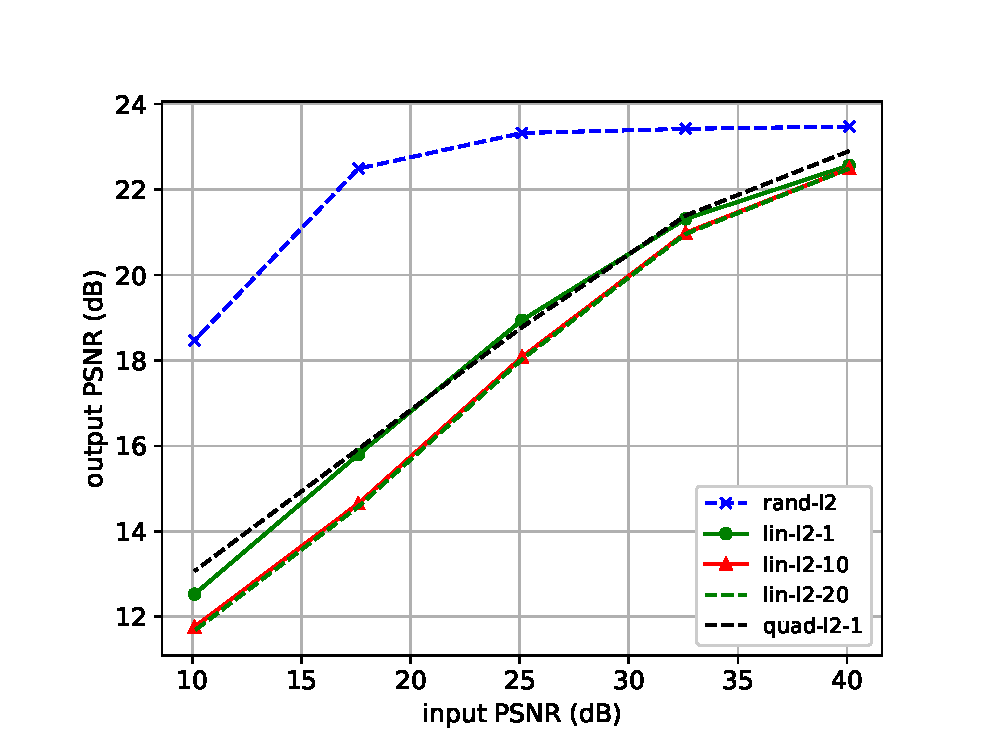
\includegraphics[width=.95\linewidth]{\detokenize{./images/figures/fcnn_fig_mnist_l2}}
		\caption{FCNN PSNR Figure ($l_2$-Norm)}
		\label{fcnn_l2_figure}
	\end{minipage}\hfill
	\begin {minipage}{0.45\textwidth}
		\centering
	 	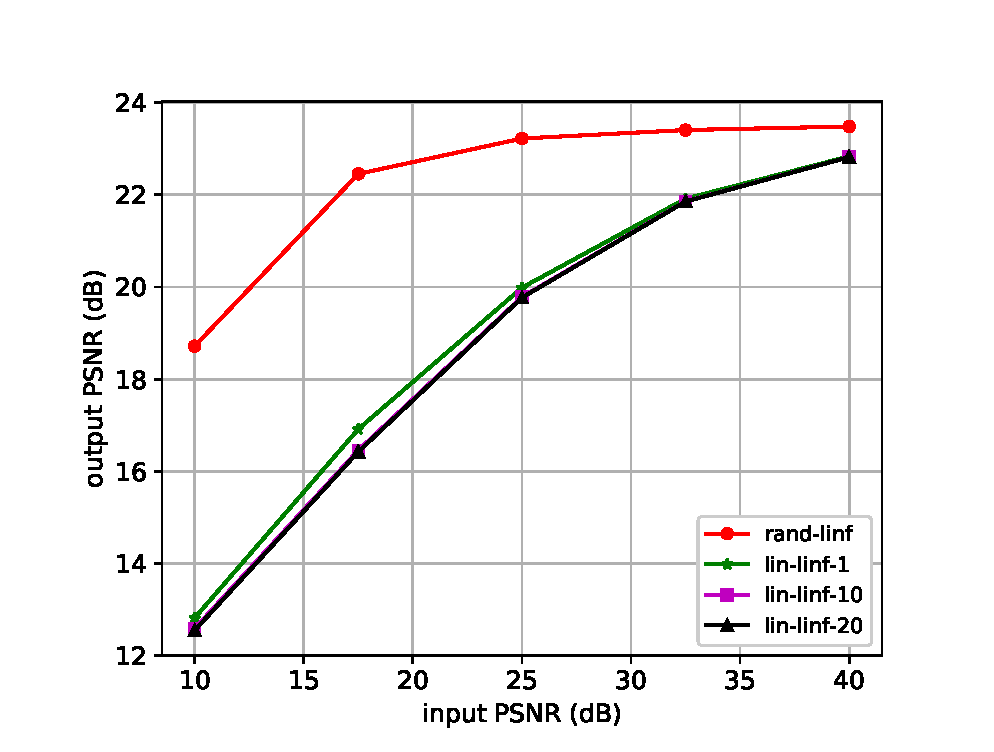
\includegraphics[width=.95\linewidth]{\detokenize{./images/figures/fcnn_fig_mnist_linf}}
		\caption{FCNN PSNR Figure ($l_\infty$-Norm)}
		\label{fcnn_linf_figure}
	\end{minipage}
\end{figure}


\begingroup
For the FCNN network \autoref{fcnn_l2_figure} and \autoref{fcnn_linf_figure} display the linear and quadratic
perturbation change under a $l_2$ and $l_\infty$ constraint. In this case,
the $l_2$-solution slightly outperforms the $l_\infty$ solution due to higher degrees
of freedom in the $l_2$-norm. The maximum output change for the FCNN network diverges around 6.5 dB from the random
benchmark under the $l_2$-norm constraint. For the $l_\infty$-norm the PSNR change is only 6 dB.
\endgroup


\begin{figure}[!htb]
	\begin{minipage}{0.45\textwidth}
		\centering
		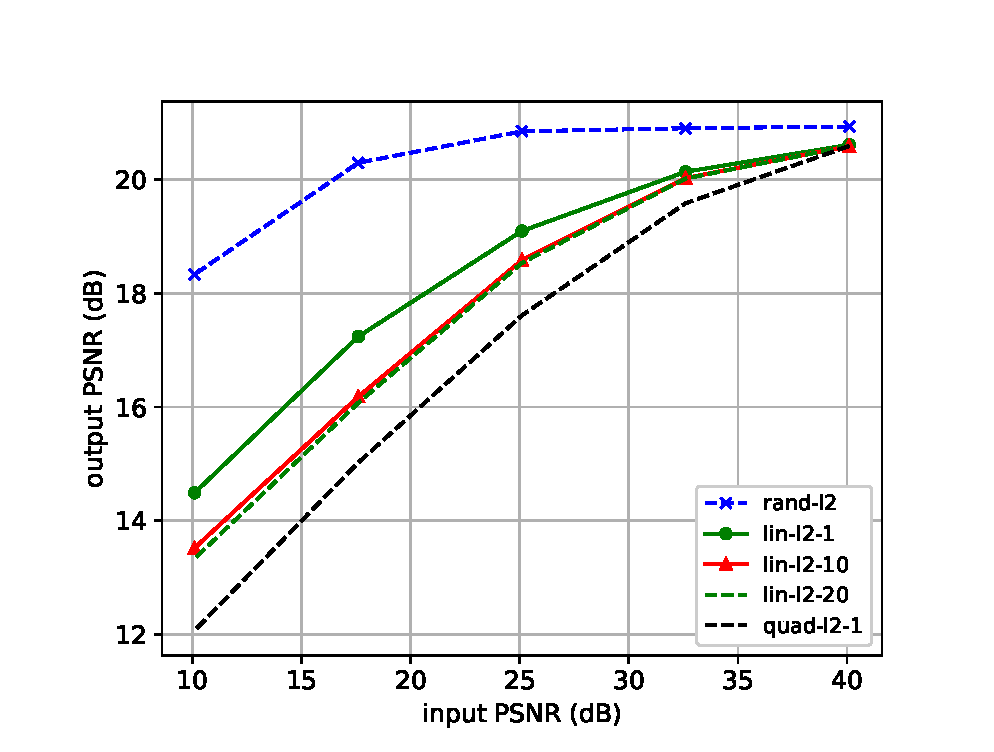
\includegraphics[width=.95\linewidth]{\detokenize{./images/figures/fcnn2_fig_mnist_l2}}
		\caption{FCNN2 PSNR Figure ($l_2$-Norm)}
		\label{fcnn2_l2_figure}
	\end{minipage}\hfill
	\begin {minipage}{0.45\textwidth}
		\centering
	 	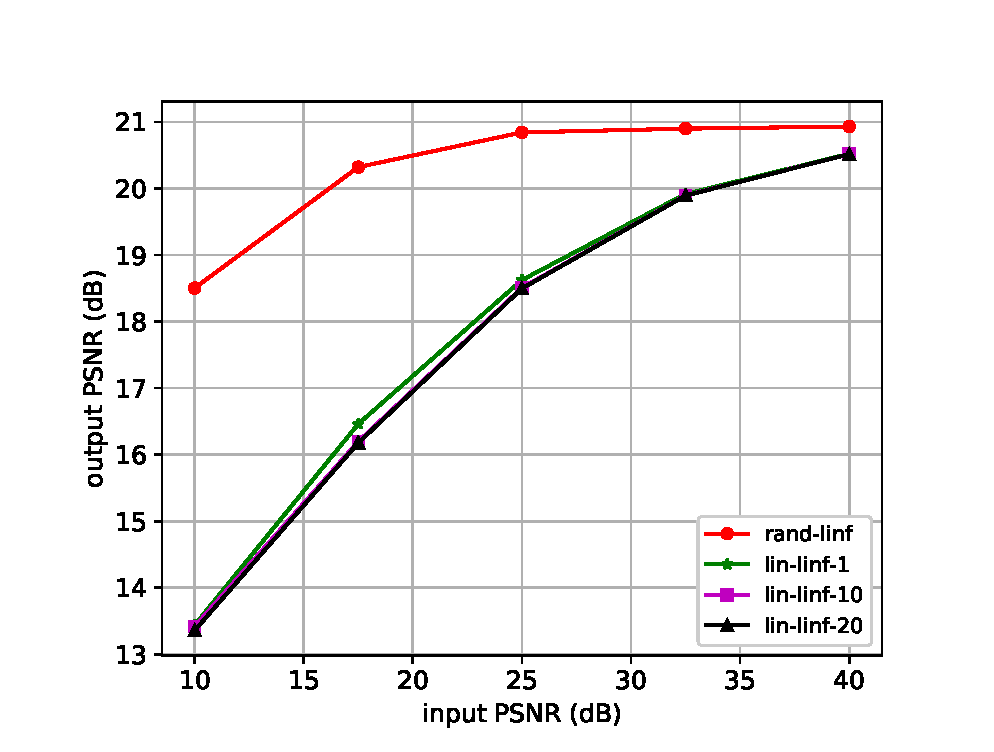
\includegraphics[width=.95\linewidth]{\detokenize{./images/figures/fcnn2_fig_mnist_linf}}
		\caption{FCNN2 PSNR Figure ($l_\infty$-Norm)}
		\label{fcnn2_linf_figure}
	\end{minipage}
\end{figure}


\begingroup
The FCNN2 network yields similar results. The best adversarial examples are provided by the quadratic solution with a 6.2 dB lower PSNR.
In contrast to the results from the FCNN network, the linear solutions provide significantly worse results than the quadratic solution. 20 iterations
of the linear closed form solution using the $l_2$ constraint are around 1 dB less effective than one iteration of the quadratic solution.
20 iterations also perform only 0.1 dB better than 10 iterations. For the $l_\infty$-norm the change between multiple iterations is even less noticable.
\endgroup

\begin{figure}[!htb]
	\begin{minipage}{0.45\textwidth}
		\centering
		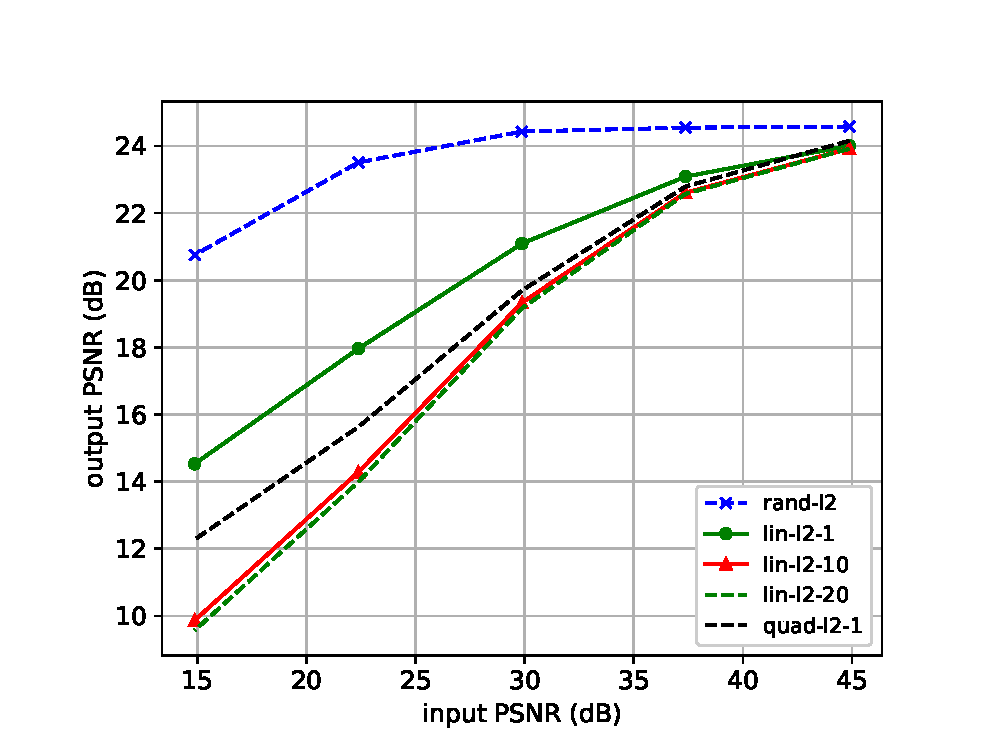
\includegraphics[width=.95\linewidth]{\detokenize{./images/figures/fcnn3_fig_cifar_l2}}
		\caption{FCNN3 PSNR Figure ($l_2$-Norm)}
		\label{fcnn3_l2_figure}
	\end{minipage}\hfill
	\begin {minipage}{0.45\textwidth}
		\centering
	 	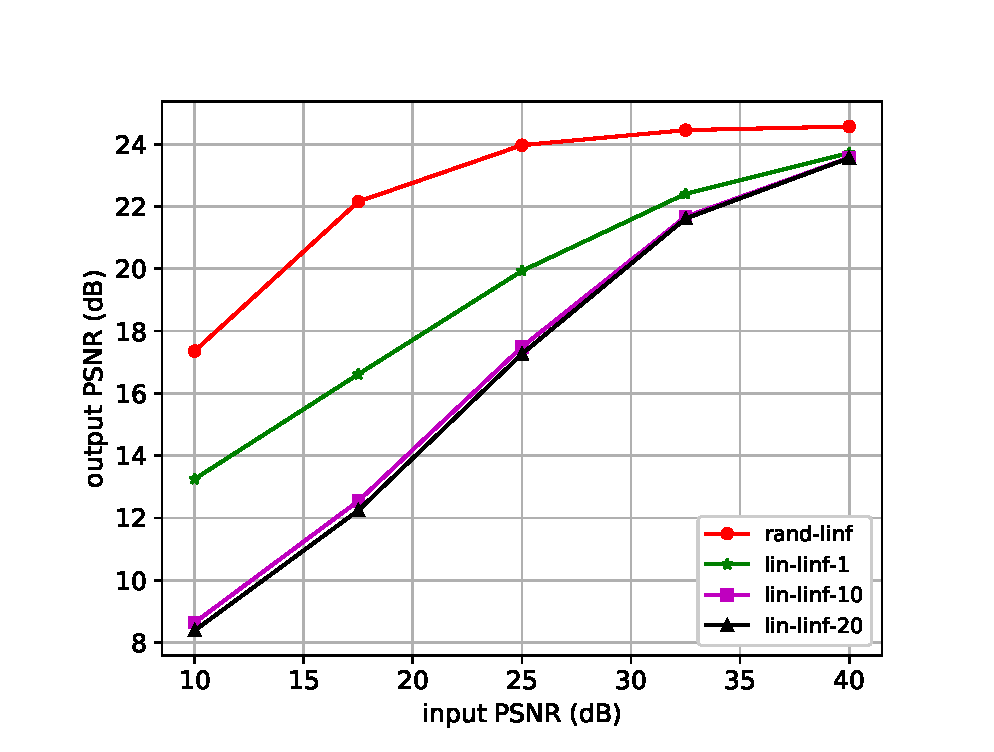
\includegraphics[width=.95\linewidth]{\detokenize{./images/figures/fcnn3_fig_cifar_linf}}
		\caption{FCNN3 PSNR Figure ($l_\infty$-Norm)}
		\label{fcnn3_linf_figure}
	\end{minipage}
\end{figure}

\begingroup
For FCNN3 the experiments' results are shown in \autoref{fcnn3_l2_figure} and \autoref{fcnn3_linf_figure}.
The maximum PSNR change from a random benchmark is 11 dB. In this case the linear solution
outperforms the quadratic solution by 2 dB for 10 and 20 iterations. The higher number of dimensions in the CIFAR
dataset seems to benefit the iterative solution. Generally, it is noticable that lower PSNR input values relate
to lower PSNR output values. This is sensible since lower PSNR values are directly connected to higher $\epsilon$ values
through the MSE.
\endgroup

\begin{figure}[!htb]
	\begin{minipage}{0.45\textwidth}
		\centering
		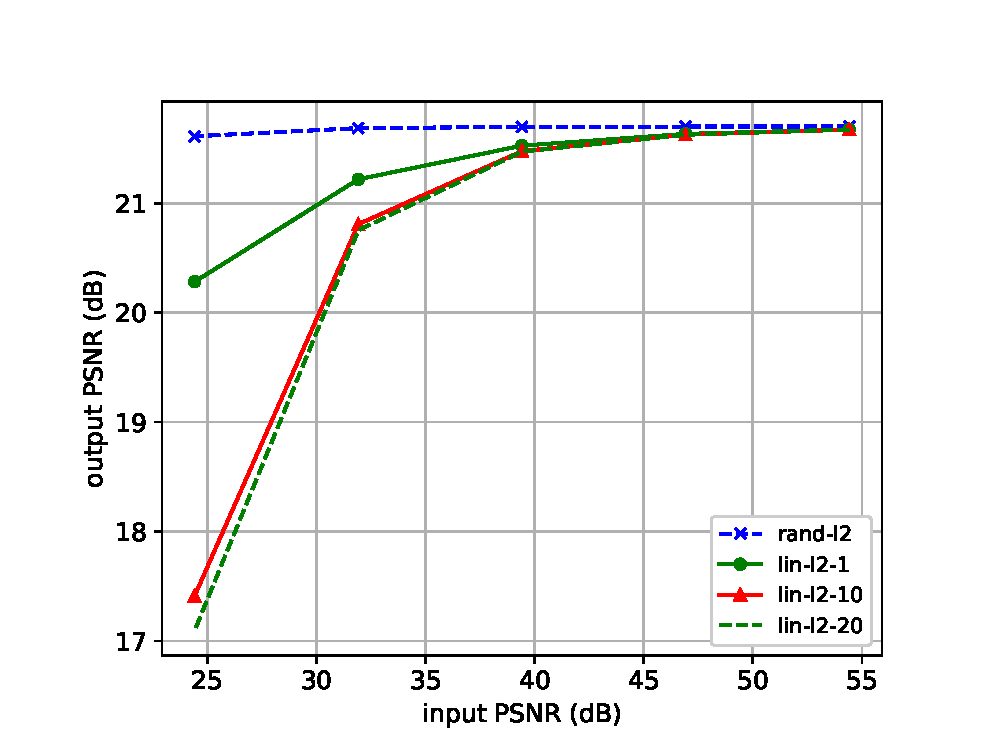
\includegraphics[width=.95\linewidth]{\detokenize{./images/figures/aen_stl10_fig_stl10_l2}}
		\caption{AEN\_STL10 PSNR Figure ($l_2$-Norm)}
		\label{aen_stl10_l2_figure}
	\end{minipage}\hfill
	\begin {minipage}{0.45\textwidth}
		\centering
	 	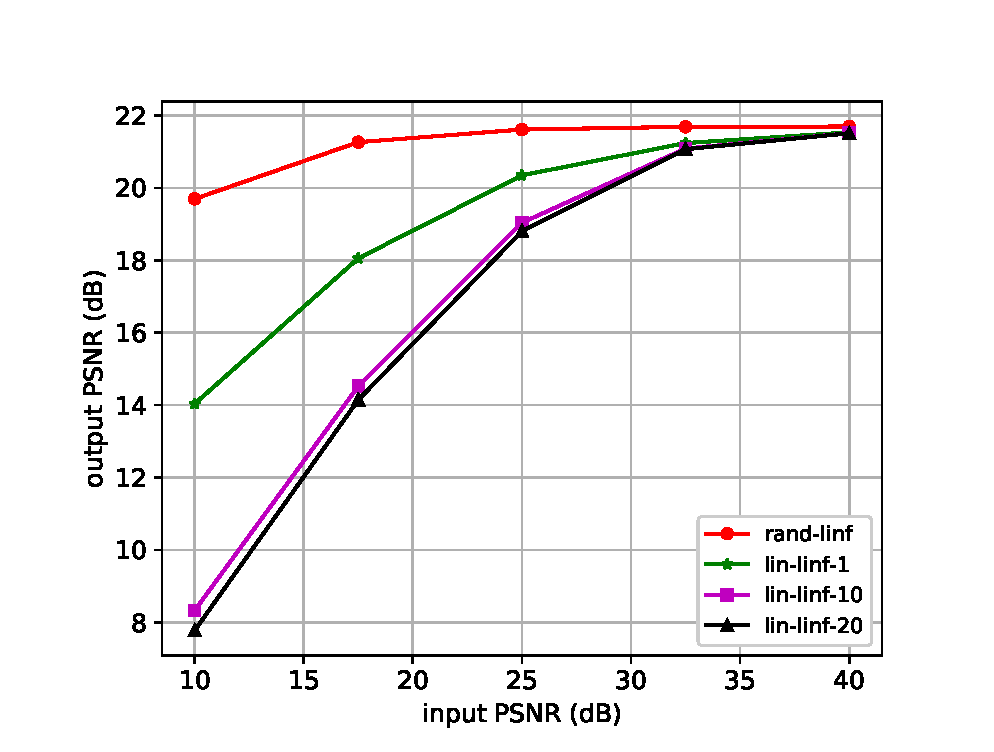
\includegraphics[width=.95\linewidth]{\detokenize{./images/figures/aen_stl10_fig_stl10_linf}}
		\caption{AEN\_STL10 PSNR Figure ($l_\infty$-Norm)}
		\label{aen_stl10_linf_figure}
	\end{minipage}
\end{figure}

\begingroup
AEN\_STL10 performs similar to previously discussed networks, but shows a rapid decline for higher $\epsilon$ values.
An input PSNR change from 25 dB to 33 dB leads to an output PSNR change of more than 3 dB.
The iterative improvement from 10 to 20 iterations is less than 0.5 dB for the $l_2$ and $l_\infty$ solution.
\endgroup


\begin{figure}[!htb]
	\begin{minipage}{0.45\textwidth}
		\centering
		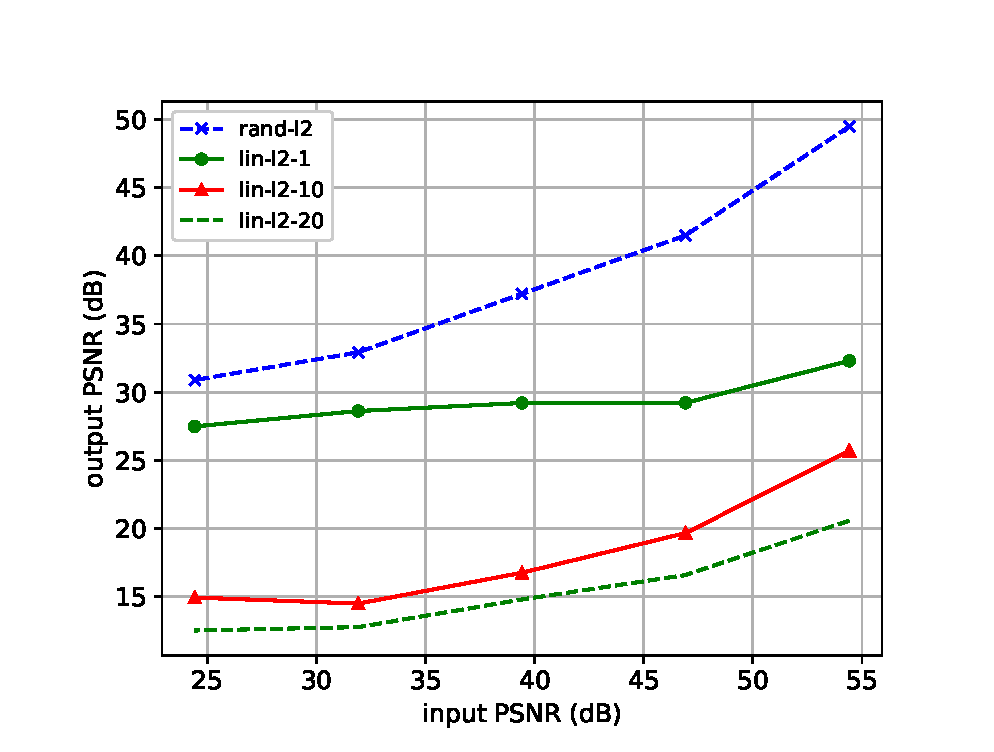
\includegraphics[width=.95\linewidth]{\detokenize{./images/figures/koala_fig_stl10_l2}}
		\caption{KOALA PSNR Figure ($l_2$-Norm)}
		\label{koala_l2_figure}
	\end{minipage}\hfill
	\begin {minipage}{0.45\textwidth}
		\centering
	 	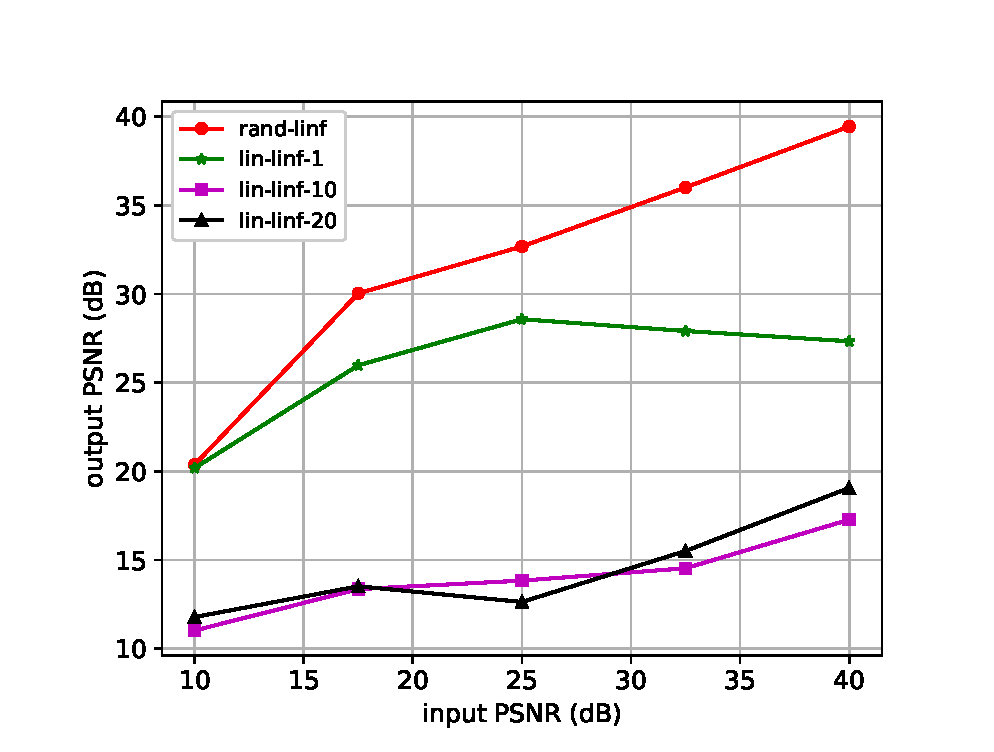
\includegraphics[width=.95\linewidth]{\detokenize{./images/figures/koala_fig_stl10_linf}}
		\caption{KOALA PSNR Figure ($l_\infty$-Norm)}
		\label{koala_linf_figure}
	\end{minipage}
\end{figure}

\begingroup
The PSNR graphs for the colorization model KOALA vary greatly from previously discussed models. Instead of an increasingly
worse output for higher $\epsilon$ values the output stagnates for $l_2$ and $l_\infty$. This is caused by merging the gray
color channel with the output layer without any modifications. Furthermore, it is noteworthy that $l_\infty$ shows some
instabilities for 10 and 20 iterations.
\endgroup

\begin{figure}[!htb]
	\begin{minipage}{0.45\textwidth}
		\centering
		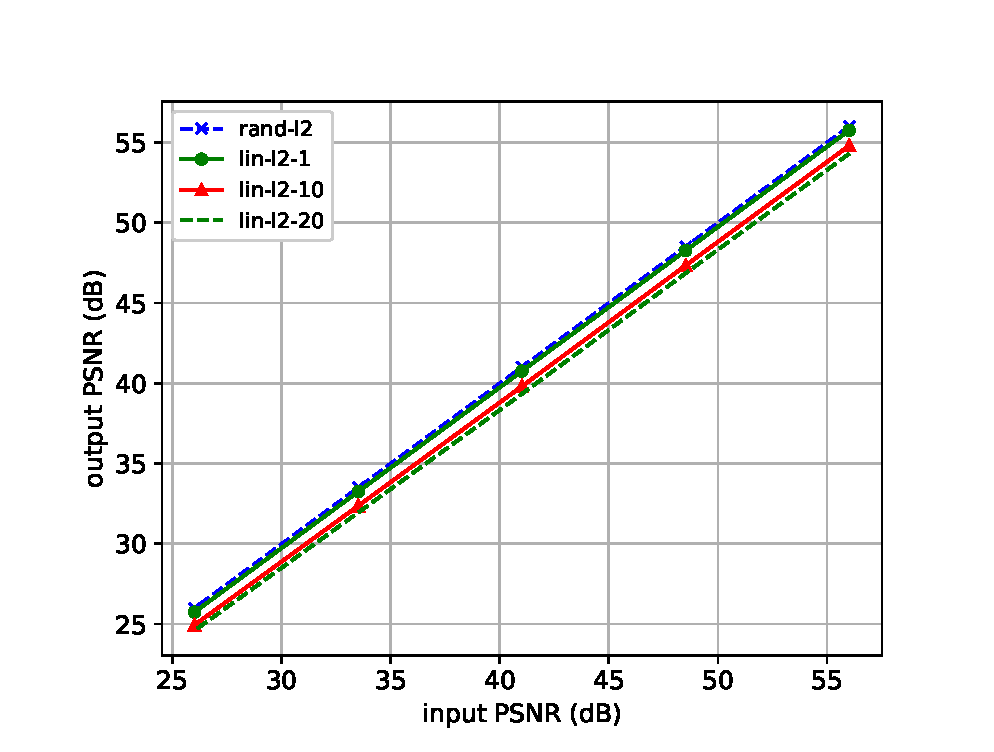
\includegraphics[width=.95\linewidth]{\detokenize{./images/figures/c_dcscn_fig_set14_l2}}
		\caption{C\_DCSCN PSNR Figure ($l_2$-Norm)}
		\label{c_dcscn_l2_figure}
	\end{minipage}\hfill
	\begin {minipage}{0.45\textwidth}
		\centering
	 	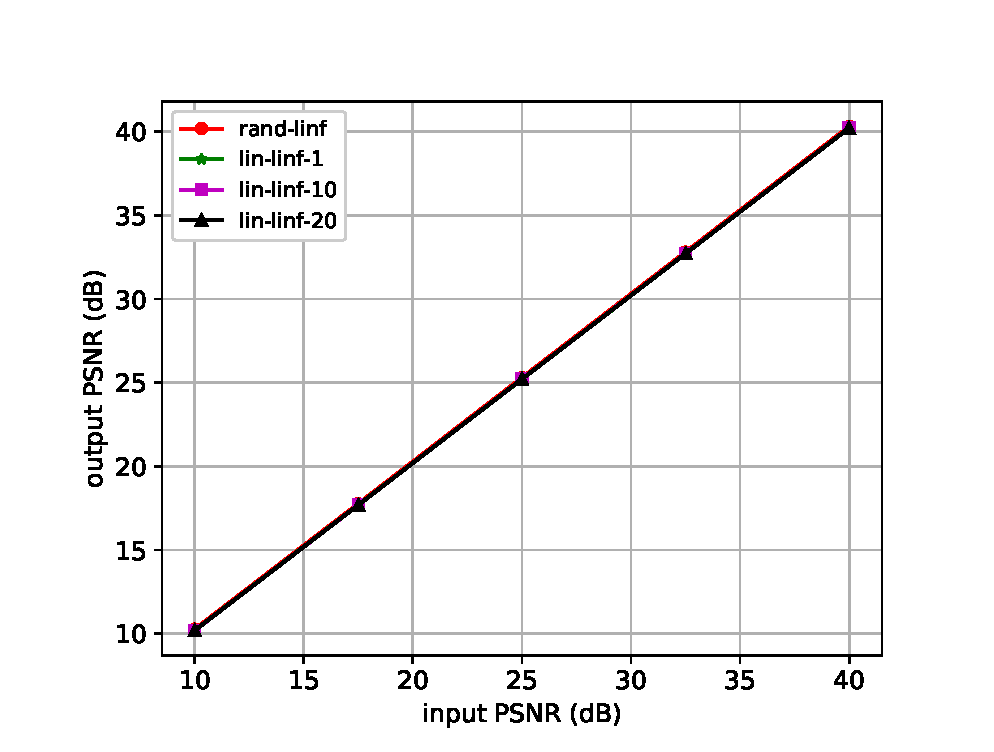
\includegraphics[width=.95\linewidth]{\detokenize{./images/figures/c_dcscn_fig_set14_linf}}
		\caption{C\_DCSCN PSNR Figure ($l_\infty$-Norm)}
		\label{c_dcscn_linf_figure}
	\end{minipage}
\end{figure}


\begingroup
Similarly to KOALA, C\_DCSCN has a relatively stable PSNR change for different $\epsilon$ values. In this case the
small impact of adversarial examples is most likely caused by the bicubic interpolation and dropout training used
in training the network. Since the DNN is only used to calculate a residual to the bicubic interpolation the impact
of adversarial examples is low.
\endgroup

\begingroup
In general, the quadratic and linear solution for 20 iterations lie within a range of 2 dB from each other. Therefore,
the impact of more than 10 iterations seems to be low. However, successive linearizations heavily improve the
performance of linear adversarial attacks. Linear solutions seem to perform better for datasets
with multiple color channels like CIFAR. The quadratic solution only performed slightly better than
the linear solution for the MNIST dataset.
Despite this fact, the quadratic solution can be performed using less iterations and can therefore yield faster results if the memory requirements for the jacobians
are met.

One of the most notable examples for the MNIST dataset is provided by \autoref{fcnn2_examples} for a PSNR
of 32.50 and the FCNN2 network. It can be observed that FCNN2 is able to denoise random input changes, but fails for linear
perturbation changes. For STL10 the most notable changes can be shown using the KOALA network in \autoref{koala_examples}.
The output images are completely distorted from the original image.
For CIFAR \autoref{fcnn3_examples} shows perturbation changes for the FCNN3 network. The example images also show that
output changes are not uniformly distributed.
\endgroup


\begin{figure}[ht] % "[t!]" placement specifier just for this example
	\centering
\includegraphics[width=.7\linewidth]{\detokenize{koala_l2_39.42_exp}}
\caption{KOALA $l_{2}$-norm Examples for PSNR of 39.42}
\label{koala_examples}
\end{figure}


\begin{figure}[ht] % "[t!]" placement specifier just for this example
	\centering
\includegraphics[width=.7\linewidth]{\detokenize{fcnn2_linf_32.50_exp}}
\caption{FCNN2 $l_{\infty}$-norm Examples for PSNR of 32.50}
\label{fcnn2_examples}
\end{figure}

\begin{figure}[ht] % "[t!]" placement specifier just for this example
	\centering
\includegraphics[width=.7\linewidth]{\detokenize{fcnn3_l2_22.37_exp}}
\caption{FCNN3 $l_{2}$-norm Examples for PSNR of 22.37}
\label{fcnn3_examples}
\end{figure}


\begingroup
Apart from strictly linear and quadratic solutions this thesis has also provided different multiple pixel attacks.
In this case $rand$-$T$, $lin$-$T$ and $pixel$-$T$ denote multiple subset attacks that change $T$ pixels.
Since all experiments were image based, subset and pixel can be used synonymously in the following paragraphs.
For $rand$-$T$ a set of pixels is randomly drawn and the values determined based on the respective norm constraint.
\autoref{fcnn_single_figure} and \autoref{fcnn2_single_figure} show multiple single pixel attacks for 100
changed subsets. Most notably the quadratic multiple subset attack performs better than the linear attack for
all chosen models and datasets. This is caused by missing iteration steps for the linear solution.
$pixel$ and $pixel$-$100$ define the different quadratic adversarial attacks. It can
be observed that a higher number of attacked subsets leads to a lower PSNR. Furthermore, higher $\epsilon$
values can be directly related to a lower PSNR. Some adversarial examples for FCNN3 are provided by
\autoref{fcnn3_single_examples}.
\endgroup


\begin{figure}[!htb]
	\begin{minipage}{0.45\textwidth}
		\centering
		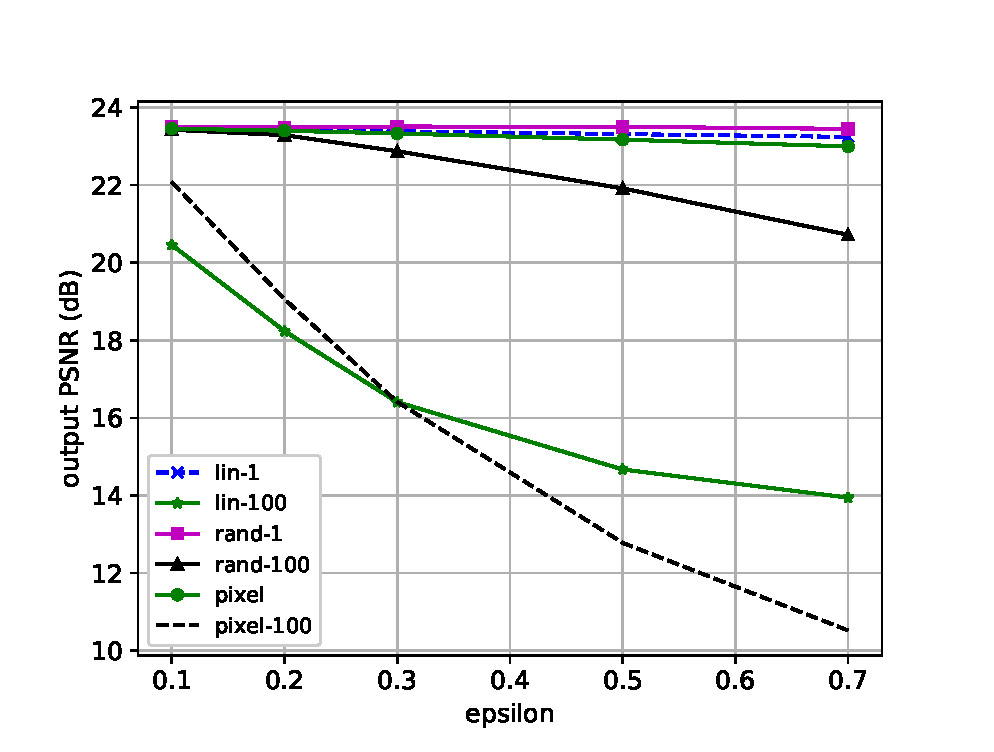
\includegraphics[width=.95\linewidth]{\detokenize{./images/figures/fcnn_fig_mnist_pixel}}
		\caption{FCNN PSNR Figure (Single Subset Attack)}
		\label{fcnn_single_figure}
	\end{minipage}\hfill
	\begin {minipage}{0.45\textwidth}
		\centering
	 	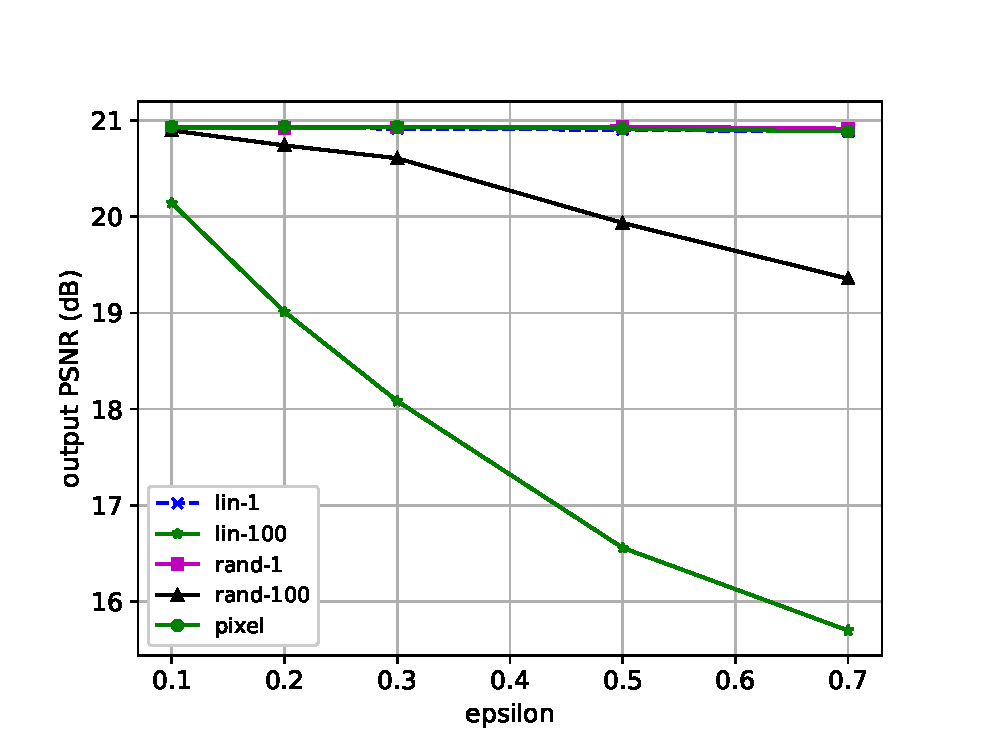
\includegraphics[width=.95\linewidth]{\detokenize{./images/figures/fcnn2_fig_mnist_pixel}}
		\caption{FCNN2 PSNR Figure (Single Subset Attack)}
		\label{fcnn2_single_figure}
	\end{minipage}
\end{figure}


\begin{figure}[ht] % "[t!]" placement specifier just for this example
	\centering
\includegraphics[width=.7\linewidth]{\detokenize{fcnn3_pixel_0.50_exp}}
\caption{FCNN3 Single Subset Attack Examples for $\epsilon = 0.50$}
\label{fcnn3_single_examples}
\end{figure}


\begingroup
Investigating the relationship between the ordering of the jacobians and output of the quadratic solution leads to
no significant change.
\autoref{single_subset_different_order} shows that ordering from the largest to the smallest jacobian is not
necessarily the best solution. The ordering for different depth sizes could possibly be improved by using a heuristic that takes the
uncertainty of $\bm{\rho}$ into account. Otherwise, there seems to be no notable difference in \autoref{single_subset_different_order} and \autoref{single_subset_different_order_2}.
The ordering of the jacobians in these figures is described in the following way:
$pixel$ (normal ordering), $pixel$-$2$ (random ordering) and $pixel$-$3$ (reverse ordering).
\endgroup

\begin{figure}[!htb]
	\begin{minipage}{0.45\textwidth}
		\centering
		\includegraphics[width=.95\linewidth]{\detokenize{fcnn3_fig_cifar_pixel-2_1}}
		\caption{FCNN3 PSNR Figure for Single Subset Attacks (1 Subset)}
		\label{single_subset_different_order}
	\end{minipage}\hfill
	\begin {minipage}{0.45\textwidth}
		\centering
	 	\includegraphics[width=.95\linewidth]{\detokenize{fcnn3_fig_cifar_pixel-2_2}}
		\caption{FCNN3 PSNR Figure for Single Subset Attacks (10 Subsets)}
		\label{single_subset_different_order_2}
	\end{minipage}
\end{figure}

\begingroup
In conclusion, the convex adversarial attacks, provided in this thesis, have proven to be effective. Especially, overtrained
FCNNs without any dropout or adversarial training performed poorly against different attacks.
With regard to the chosen architecture, convolutional networks like FCNN2 showed slightly more resilience against
adversarial examples.
Unfortunately, it is often difficult to draw conclusions
from only a small set of models. Therefore, further research needs to go into analyzing if convolutional networks are truly
less susceptible to these attacks. It is also unclear if regression problems can be directly related to autoencoders.
\endgroup

\chapter{Conclusion and Outlook}\label{sec:section}

\begingroup
In this thesis, various adversarial attacks were theoretically and practically evaluated. Comparisons
between previous research and methods introduced in this thesis were drawn.
The simulation results have clearly shown that neural networks
are not resistant to adversarial attacks. Large changes in output images were discovered with only small perturbation
changes to the input. Iterative techniques have proven to significantly improve adversarial perturbation attacks. Noteworty
performance increases were found for less than 10 iterations.
Despite this fact, this thesis also shows that networks can be adjusted to remove
the impact of adversarial attacks. Techniques to avoid adversarial attacks include dropout, training with FGSM or using
a predefined filter like the bicubic interpolation filter in the C\_DCSCN model. In a more general
scenario of non-autoencoders these attacks can be used to change the output of regression problems.
The application of these techniques was introduced through the paper Eykholt et al. \cite{RealWorld}.

Besides the mere implementation of adversarial attacks, this thesis has also given an introduction into different
convex optimization techniques. Older literature like Goodfellow et al. \cite{Goodfellow} was introduced
and used to derive newer techniques like single subset attacks or various generalization provided by
Balda et al. \cite{NeuralError}. Specifically this thesis has given a look into the inner workings of optimization
techniques and provides various proofs used to calculate adversarial examples. For single subset
attacks the impact of ordering for a greedy approximation was also studied.
The adversarial attacks themselves were studied based on six different neural networks. These networks utilize
convolutional and fully-connected layers to solve their respective regression problem. The most resistant network
has proven to be the residual network (C\_DCSCN), which only uses a DNN for slight
variations of a higher resolution image.

Apart from using convex optimization techniques to find adversarial examples it is also possible to build
Generative Adversarial Networks (GANs) that are trained to find adversarial examples for a certain type
of network. Due to their higher non-linearity they might be able to find adversarial examples, which cannot be
found due to the taylor approximations used for convex optimizations \cite{GAN}. Evaluating the effectiveness of
these attacks against convex solutions is left for future research.
\endgroup


\newpage

\chapter*{Appendix}\label{sec:appendix}
\addcontentsline{toc}{chapter}{Appendix}
\markboth{Appendix}{Appendix}

%%% l2 norm results

\begin{figure}[ht] % "[t!]" placement specifier just for this example
	\centering
\includegraphics[width=.7\linewidth]{\detokenize{./images/compact/fcnn_l2_17.60}}
\caption{FCNN Example Images ($l_2$-Norm) \\ with an input PSNR of 17.60} \label{fig:e}

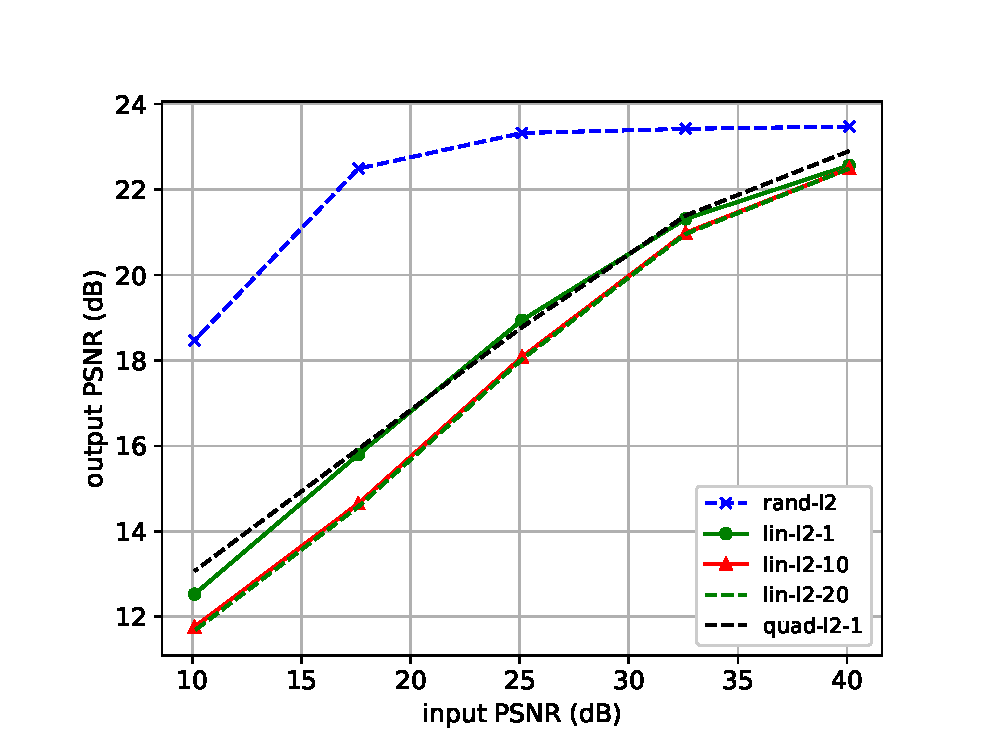
\includegraphics[width=.7\linewidth]{\detokenize{./images/figures/fcnn_fig_mnist_l2}}
\caption{FCNN PSNR Figure ($l_2$-Norm)} \label{fig:f}
\end{figure}


\begin{figure}[ht]
	\centering
\includegraphics[width=.7\linewidth]{\detokenize{./images/compact/fcnn2_l2_17.60}}
\caption{FCNN2 Example Images ($l_2$-Norm) \\ with an input PSNR of 17.60} \label{fig:e}

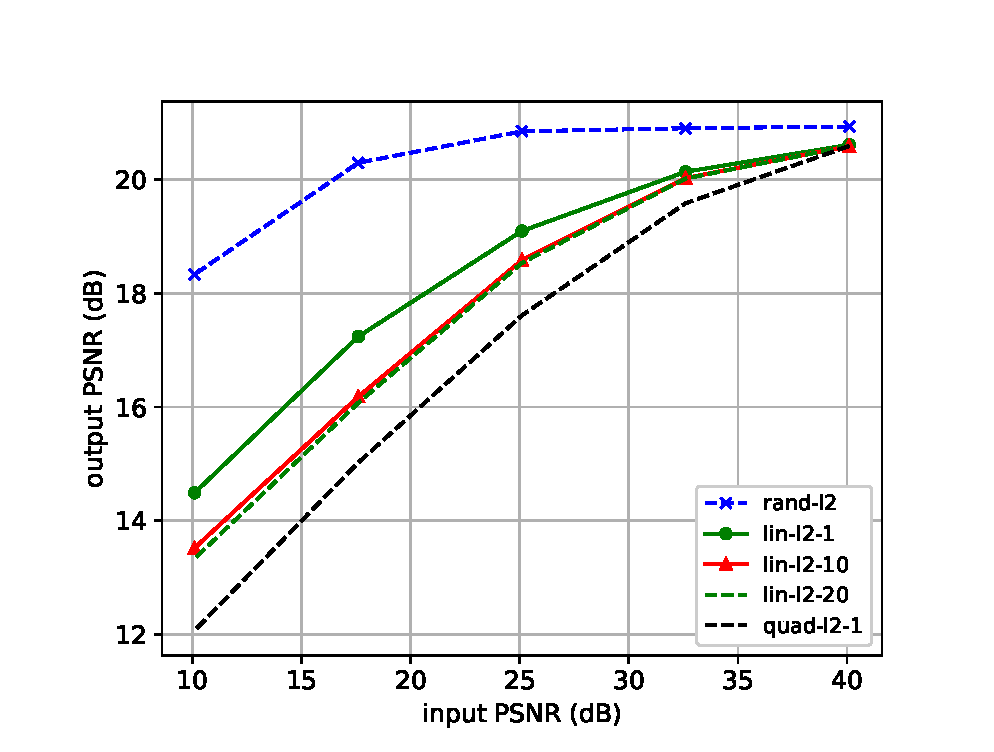
\includegraphics[width=.7\linewidth]{\detokenize{./images/figures/fcnn2_fig_mnist_l2}}
\caption{FCNN2 PSNR Figure ($l_2$-Norm)} \label{fig:f}
\end{figure}


\begin{figure}[ht]
	\centering
\includegraphics[width=.7\linewidth]{\detokenize{./images/compact/fcnn3_l2_14.87}}
\caption{FCNN3 Example Images ($l_2$-Norm) \\ with an input PSNR of 14.87} \label{fig:e}

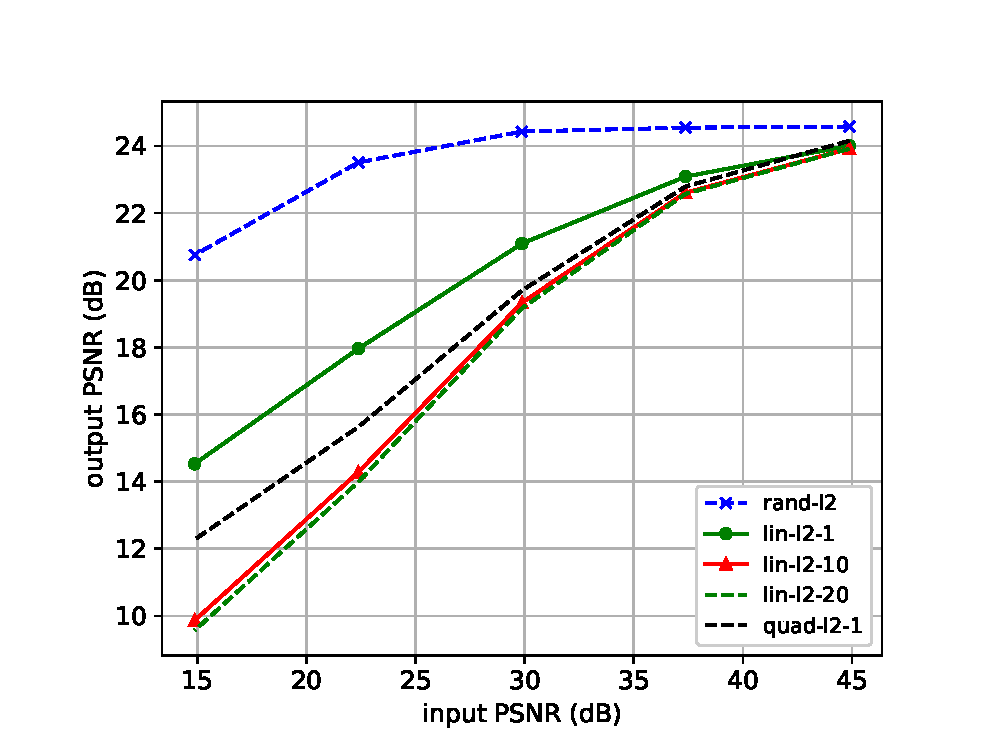
\includegraphics[width=.7\linewidth]{\detokenize{./images/figures/fcnn3_fig_cifar_l2}}
\caption{FCNN3 PSNR Figure ($l_2$-Norm)} \label{fig:fcnn3_l2}
\end{figure}


\begin{figure}[ht]
	\centering
\includegraphics[width=.7\linewidth]{\detokenize{./images/compact/aen_stl10_l2_31.92}}
\caption{AEN\_STL10 Example Images ($l_2$-Norm) \\ with an input PSNR of 31.92} \label{fig:e}

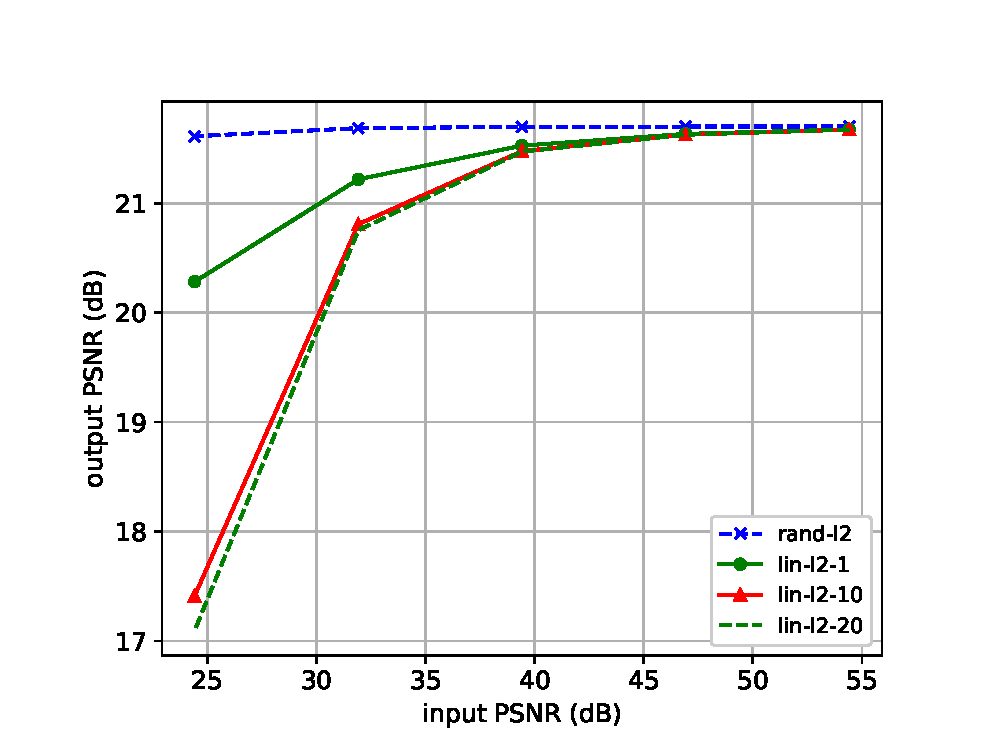
\includegraphics[width=.7\linewidth]{\detokenize{./images/figures/aen_stl10_fig_stl10_l2}}
\caption{AEN\_STL10 PSNR Figure ($l_2$-Norm)} \label{fig:f}
\end{figure}


\begin{figure}[ht]
	\centering
\includegraphics[width=.7\linewidth]{\detokenize{./images/compact/koala_l2_31.92}}
\caption{KOALA Example Images ($l_2$-Norm) \\ with an input PSNR of 31.92} \label{fig:e}

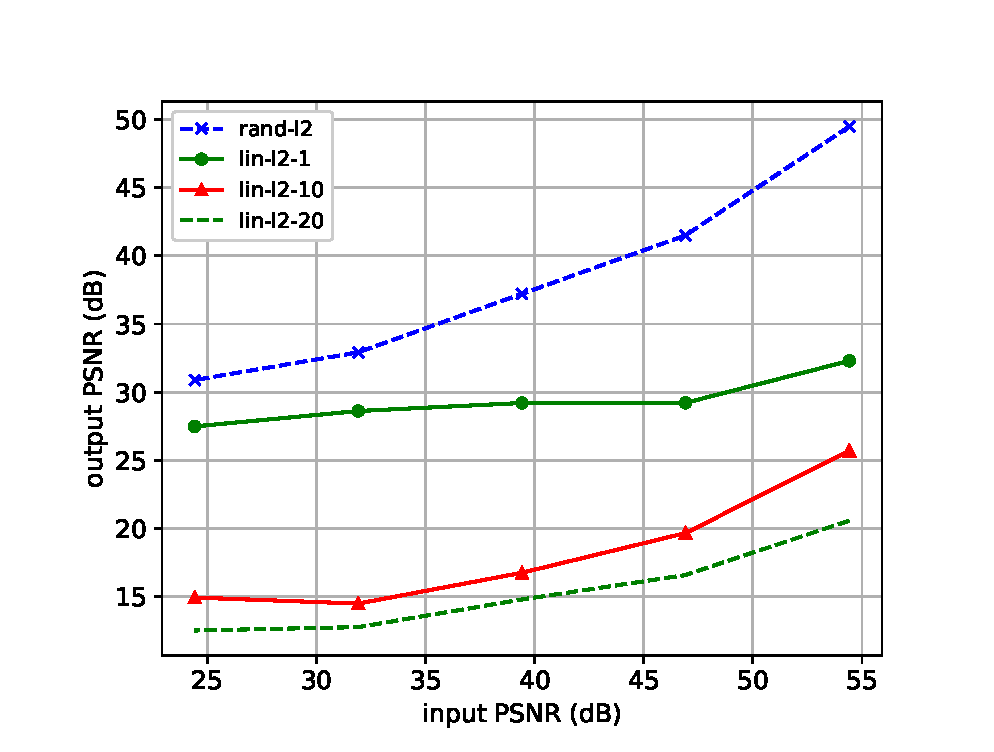
\includegraphics[width=.7\linewidth]{\detokenize{./images/figures/koala_fig_stl10_l2}}
\caption{KOALA PSNR Figure ($l_2$-Norm)} \label{fig:f}
\end{figure}


\begin{figure}[ht]
	\centering
\includegraphics[width=.7\linewidth]{\detokenize{./images/compact/c_dcscn_l2_26.02}}
\caption{C\_DCSCN Example Images ($l_2$-Norm) \\ with an input PSNR of 26.02} \label{fig:e}

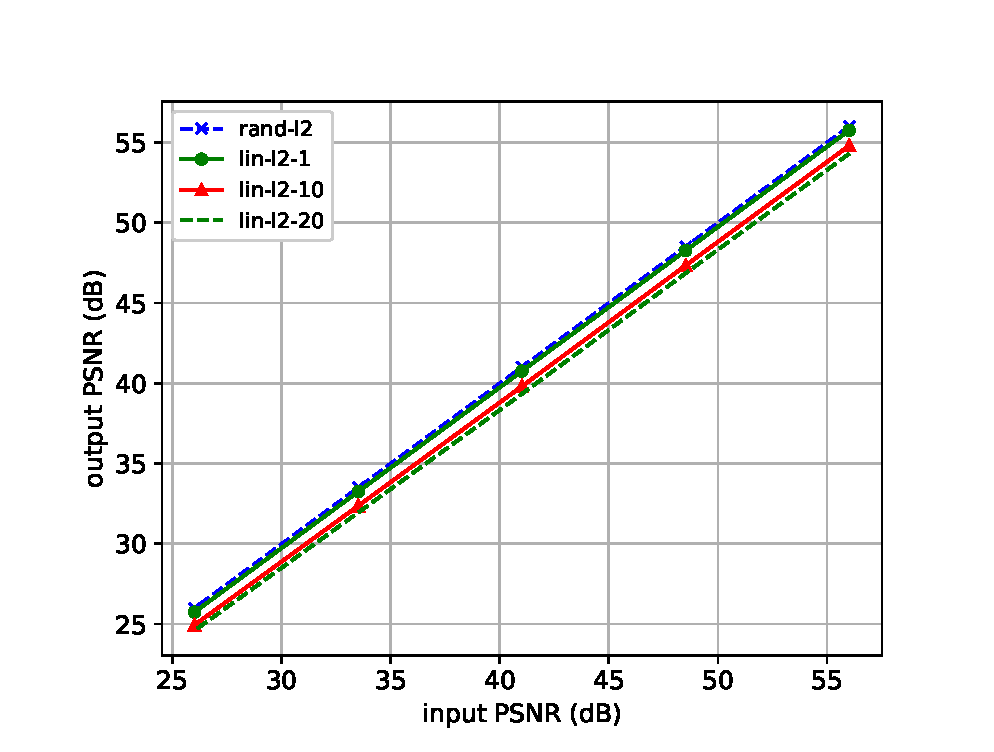
\includegraphics[width=.7\linewidth]{\detokenize{./images/figures/c_dcscn_fig_set14_l2}}
\caption{C\_DCSCN PSNR Figure ($l_2$-Norm)} \label{fig:f}
\end{figure}

%%% linf norm results

\begin{figure}[ht]
	\centering
\includegraphics[width=.7\linewidth]{\detokenize{./images/compact/fcnn_linf_17.50}}
\caption{FCNN Example Images ($l_\infty$-Norm) \\ with an input PSNR of 17.50} \label{fig:e}

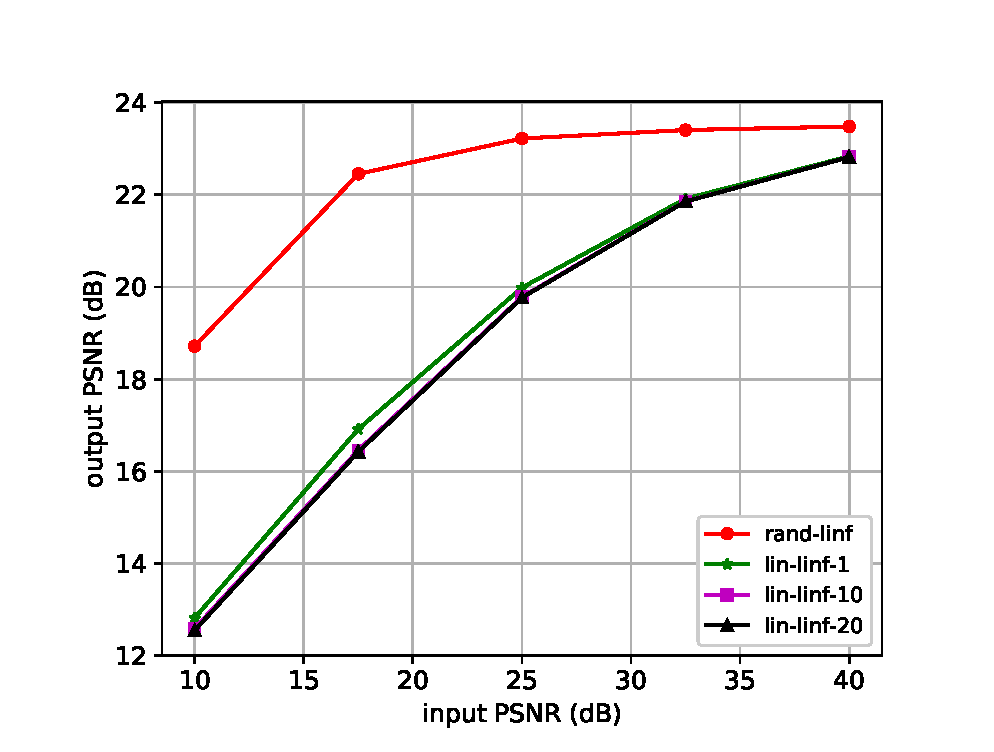
\includegraphics[width=.7\linewidth]{\detokenize{./images/figures/fcnn_fig_mnist_linf}}
\caption{FCNN PSNR Figure ($l_\infty$-Norm)} \label{fig:f}
\end{figure}

\begin{figure}[ht]
	\centering
\includegraphics[width=.7\linewidth]{\detokenize{./images/compact/fcnn2_linf_17.50}}
\caption{FCNN2 Example Images ($l_\infty$-Norm) \\ with an input PSNR of 17.50} \label{fig:e}

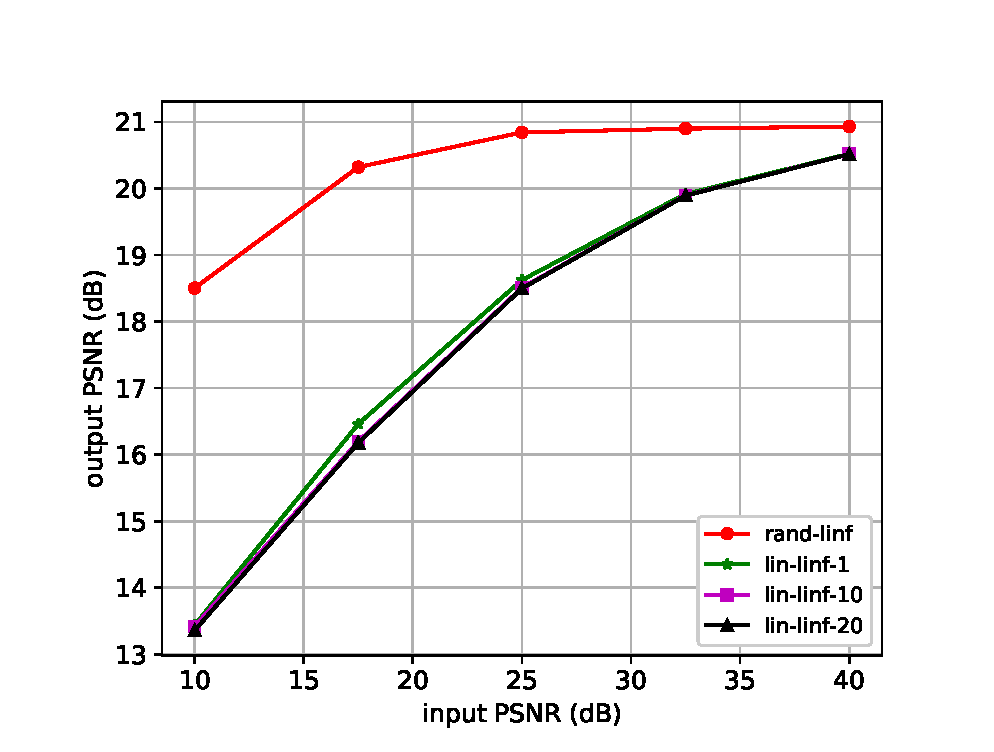
\includegraphics[width=.7\linewidth]{\detokenize{./images/figures/fcnn2_fig_mnist_linf}}
\caption{FCNN2 PSNR Figure ($l_\infty$-Norm)} \label{fig:f}
\end{figure}

\begin{figure}[ht]
	\centering
\includegraphics[width=.7\linewidth]{\detokenize{./images/compact/fcnn3_linf_17.50}}
\caption{FCNN3 Example Images ($l_\infty$-Norm) \\ with an input PSNR of 17.50} \label{fig:e}

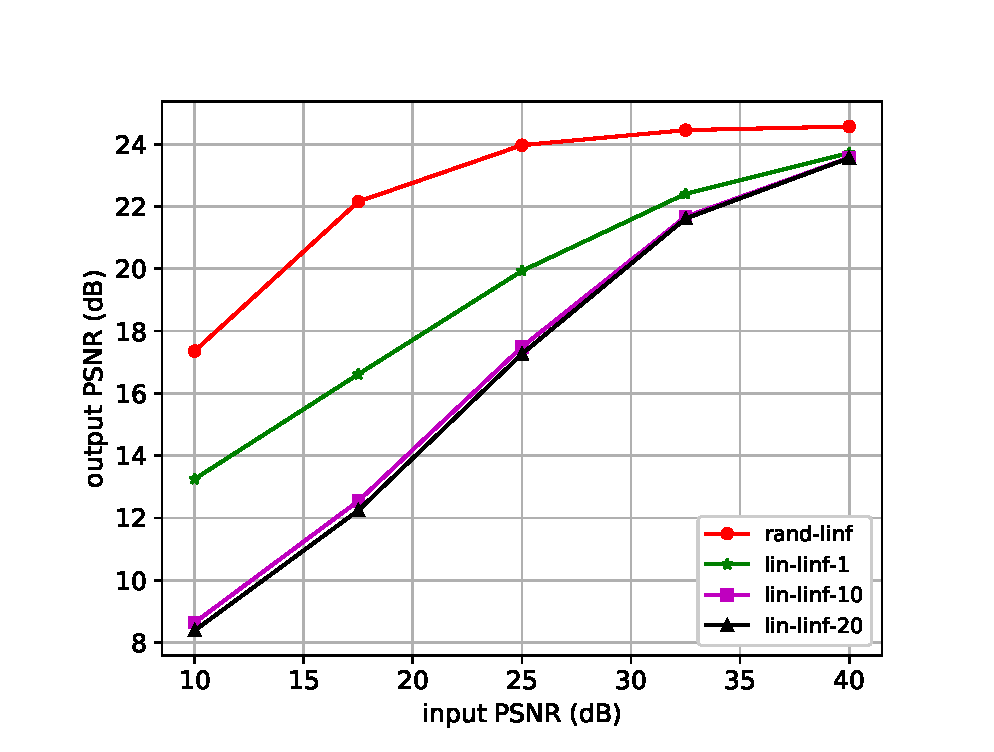
\includegraphics[width=.7\linewidth]{\detokenize{./images/figures/fcnn3_fig_cifar_linf}}
\caption{FCNN3 PSNR Figure ($l_\infty$-Norm)} \label{fig:f}
\end{figure}

\begin{figure}[ht]
	\centering
\includegraphics[width=.7\linewidth]{\detokenize{./images/compact/aen_stl10_linf_17.50}}
\caption{AEN\_STL10 Example Images ($l_\infty$-Norm) \\ with an input PSNR of 17.50} \label{fig:e}

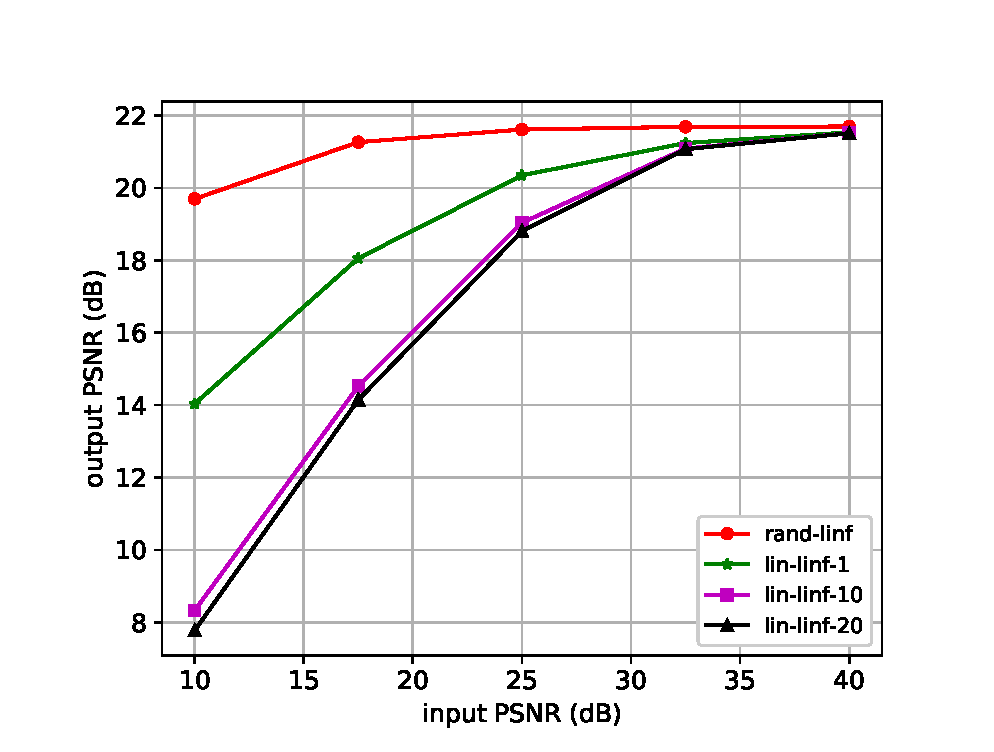
\includegraphics[width=.7\linewidth]{\detokenize{./images/figures/aen_stl10_fig_stl10_linf}}
\caption{AEN\_STL10 PSNR Figure ($l_\infty$-Norm)} \label{fig:f}
\end{figure}

\begin{figure}[ht]
	\centering
\includegraphics[width=.7\linewidth]{\detokenize{./images/compact/koala_linf_17.50}}
\caption{KOALA Example Images ($l_\infty$-Norm) \\ with an input PSNR of 17.50} \label{fig:e}

\includegraphics[width=.7\linewidth]{\detokenize{./images/figures/koala_fig_stl10_linf}}
\caption{KOALA PSNR Figure ($l_\infty$-Norm)} \label{fig:f}
\end{figure}

\begin{figure}[ht]
	\centering
\includegraphics[width=.7\linewidth]{\detokenize{./images/compact/c_dcscn_linf_17.50}}
\caption{C\_DCSCN Example Images ($l_\infty$-Norm) \\ with an input PSNR of 17.50} \label{fig:e}

\includegraphics[width=.7\linewidth]{\detokenize{./images/figures/c_dcscn_fig_set14_linf}}
\caption{C\_DCSCN PSNR Figure ($l_\infty$-Norm)} \label{fig:f}
\end{figure}

%% pixel attack

\begin{figure}[ht]
	\centering
\includegraphics[width=.7\linewidth]{\detokenize{./images/compact/fcnn_pixel_0.20}}
\caption{FCNN Example Images \\ with an input $\epsilon \;$ of 0.20} \label{fig:e}

\includegraphics[width=.7\linewidth]{\detokenize{./images/figures/fcnn_fig_mnist_pixel}}
\caption{FCNN PSNR Figure (Single Subset Attack)} \label{fig:f}
\end{figure}

\begin{figure}[ht]
	\centering
\includegraphics[width=.7\linewidth]{\detokenize{./images/compact/fcnn2_pixel_0.20}}
\caption{FCNN2 Example Images \\ with an input $\epsilon \;$ of 0.20} \label{fig:e}

\includegraphics[width=.7\linewidth]{\detokenize{./images/figures/fcnn2_fig_mnist_pixel}}
\caption{FCNN2 PSNR Figure (Single Subset Attack)} \label{fig:f}
\end{figure}

\begin{figure}[ht]
	\centering
\includegraphics[width=.7\linewidth]{\detokenize{./images/compact/fcnn3_pixel_0.20}}
\caption{FCNN3 Example Images \\ with an input $\epsilon \;$ of 0.20} \label{fig:e}

\includegraphics[width=.7\linewidth]{\detokenize{./images/figures/fcnn3_fig_cifar_pixel}}
\caption{FCNN3 PSNR Figure (Single Subset Attack)} \label{fig:f}
\end{figure}

\begin{figure}[ht]
	\centering
\includegraphics[width=.7\linewidth]{\detokenize{./images/compact/aen_stl10_pixel_0.20}}
\caption{AEN\_STL10 Example Images \\ with an input $\epsilon \;$ of 0.20} \label{fig:e}

\includegraphics[width=.7\linewidth]{\detokenize{./images/figures/aen_stl10_fig_stl10_pixel}}
\caption{AEN\_STL10 PSNR Figure (Single Subset Attack)} \label{fig:f}
\end{figure}

\begin{figure}[ht]
	\centering
\includegraphics[width=.7\linewidth]{\detokenize{./images/compact/koala_pixel_0.20}}
\caption{KOALA Example Images \\ with an input $\epsilon \;$ of 0.20} \label{fig:e}

\includegraphics[width=.7\linewidth]{\detokenize{./images/figures/koala_fig_stl10_pixel}}
\caption{KOALA PSNR Figure (Single Subset Attack)} \label{fig:f}
\end{figure}


\appendix
%\bibliographystyle{alpha}
%\bibliographystyle{science}
%\bibliographystyle{acm}
\bibliographystyle{IEEEtranS}
\bibliography{collection}
%\newpage
%\printindex


\end{document}
